%% This document is created by 
%% Dr. Putu Harry Gunawan
%% Template untuk Proposal TA 1 dan TA
%% Template ini digunakan untuk penulisan proposal TA 1 atau TA Fakultas Informatika, Telkom University.

\documentclass[a4paper,12pt,oneside]{book}
\usepackage[utf8]{inputenc}
\usepackage{sectsty}
\usepackage{graphicx}
\usepackage{epstopdf}
\usepackage{algorithm}
\usepackage{algpseudocode}
\usepackage{array}
\usepackage[table]{xcolor}
\usepackage{anysize}
\usepackage{amsmath}
\usepackage{amssymb}
\usepackage[indonesian]{babel}
\usepackage{indentfirst} %Spasi untuk paragraf pertama
\usepackage{geometry}
\usepackage{multirow}% http://ctan.org/pkg/multirow
\usepackage{hhline}% http://ctan.org/pkg/hhline
\marginsize{4cm}{3cm}{3cm}{3cm} %{left}{right}{top}{bottom}
\usepackage[compact]{titlesec} 
\usepackage{etoolbox}

\makeatletter
\patchcmd{\ttlh@hang}{\parindent\z@}{\parindent\z@\leavevmode}{}{}
\patchcmd{\ttlh@hang}{\noindent}{}{}{}
\makeatother

\chapterfont{\centering}
\newcommand{\bigsize}{\fontsize{16pt}{14pt}\selectfont}
\chapterfont{\centering\bigsize\bfseries}
\sectionfont{\large\bfseries}
\usepackage{tikz}
\usetikzlibrary{shapes.geometric, arrows}
%\renewcommand{\chaptertitle}{BAB}
\renewcommand{\thechapter}{\Roman{chapter}}
\renewcommand\thesection{\arabic{chapter}.\arabic{section}}
\renewcommand\thesubsection{\thesection.\arabic{subsection}}
\renewcommand{\theequation}{\arabic{chapter}.\arabic{equation}}
\renewcommand{\thefigure}{\arabic{chapter}.\arabic{figure}}
\renewcommand{\thetable}{\arabic{chapter}.\arabic{table}}

\renewcommand\bibname{Daftar Pustaka}
\addto{\captionsbahasa}{\renewcommand{\bibname}{Daftar Pustaka}}
\usepackage{fancyhdr}
\pagestyle{fancy}
\lhead{}
\chead{}
\rhead{}
\lfoot{}
\cfoot{\thepage}
\rfoot{}
\renewcommand{\headrulewidth}{0pt}

\makeatletter

%%%%%%%%%%%%%%%%%%%%%%%%%%%%%%%%%%%%%%%%%%%%%%%%%%%%%%%%%%%%
%
%  Berikut adalah data-data yang wajib diisi oleh mahasiswa
%
%%%%%%%%%%%%%%%%%%%%%%%%%%%%%%%%%%%%%%%%%%%%%%%%%%%%%%%%%%%%

\title{Pengawasan Detak Jantung dan Peringatan Aritmia secara Ubiquitous Menggunakan Protokol MQTT}\let\Title\@title   %Judul dalam bahasa Indonesia

\newcommand{\EngTitle}{Ubiquitous Heart Rate Monitoring and Arrhythmia Alerting using MQTT protocol}  %Judul dalam bahasa Inggris

\author{Muhammad Alif Akbar}  \let\Author\@author  %Nama mhs
\newcommand{\NIM}{1103132163}
\newcommand{\Prodi}{Teknik Informatika}
\newcommand{\KK}{Telematics} %UNTUK TA
\newcommand{\Gelar}{Teknik Informatika} % UNTUK TA
\date{2017}           \let\Date\@date %Maskkan hanya tahun saja
\newcommand{\Tanggal}{1} % Tanggal Pengesahan
\newcommand{\Bulan}{Agustus} % Bulan Pengesahan
\newcommand{\PembimbingSatu}{Satria Mandala, S.T, M.Sc, Ph.D}
\newcommand{\NIPPembimbingSatu}{15731897-3}
\newcommand{\Kaprodi}{Ir. Moch. Arif Bijaksana, M.Tech, Ph.D}
\newcommand{\NIPKaprodi}{03650312-4}
\newif\iflogTA
\logTAtrue   %%%%%% WARNING kode ini diaktifkan untuk format TUGAS AKHIR
\makeatother
\linespread{1}


\begin{document}
\pagenumbering{roman} 
%%\maketitle
\begin{titlepage}
\thispagestyle{empty}
%\vspace*{0.7cm}
{\centering
\large
{\bigsize\bf \Title}\\
\vspace{ 2cm}
\rm
\iflogTA
\textbf{Tugas Akhir}\\
\vspace{0.5 cm}
\textbf{Kelompok Keahlian: \KK}\\
\else
\textbf{Proposal Tugas Akhir}\\
\vspace{0.5 cm}
\textbf{Kelas TA 1}\\
\fi
\vspace{0.5 cm}
\textbf{\Author}\\ \textbf{NIM: \NIM}\\ 

\vspace{1.5 cm}

\begin{figure}[h]
{\centering {
\includegraphics[scale=0.17]{Tel-U-Logo}}\par}
\end{figure}

\vspace{2 cm}
{\bigsize\textbf{Program Studi Sarjana \Prodi}\\
\vspace{0.5 cm}
\textbf{Fakultas Informatika}\\
\vspace{0.5 cm}
\textbf{Universitas Telkom}\\
\vspace{0.5 cm}
\textbf{Bandung}\\
\vspace{0.5 cm}
\textbf{\Date}\\}
}
\pagebreak
\thispagestyle{empty}
{\centering
\iflogTA
\textbf{\large Lembar Pengesahan}\\  %UNTUK TA
\else
\textbf{\large Lembar Persetujuan}\\
\fi
\vspace{0.5cm}
\textbf{\Title}\\
\vspace{0.5cm}
\textbf{\textit{\EngTitle}}\\
\vspace{0.5cm}
\textbf{\Author}\\
\textbf{NIM: \NIM}\\
\vspace{1cm}

\iflogTA 
{ Tugas Akhir ini diterima dan disahkan untuk memenuhi sebagian dari syarat untuk memperoleh gelar sarjana \Gelar\\ Program Studi Sarjana \Prodi\\ Fakultas Informatika Universitas Telkom}\\  %% UNTUK TA
\else
{ Proposal ini diajukan sebagai usulan pembuatan tugas akhir pada\\ Program Studi Sarjana \Prodi\\ Fakultas Informatika Universitas Telkom}\\
\fi
\vspace{0.5cm}

{Bandung, \Tanggal\quad \Bulan \quad \Date}\\
{Menyetujui}\\

\vspace{0.5cm}
\iflogTA
\begin{center}
\begin{tabular}{  m{8cm}  m{8cm} }
Pembimbing 1 & Pembimbing 2
\end{tabular}
\end{center}
\else
\begin{center}
\begin{tabular}{  m{8cm}  m{8cm} }
Calon Pembimbing 1 & Calon Pembimbing 2
\end{tabular}
\end{center}
\fi
\begin{center}
\vspace{2cm}
\begin{tabular}{  m{8cm}  m{8cm} }
\underline{\PembimbingSatu} & \underline{\PembimbingDua} \\ 
NIP: \NIPPembimbingSatu & NIP: \NIPPembimbingDua
\end{tabular}
\end{center}
\vspace{0.5cm}
\iflogTA
Mengesahkan,\\   %% UNTUK TA
Kepala Program Studi \Prodi\\ %% UNTUK TA
\vspace{2.5cm}   %% UNTUK TA
\underline{\Kaprodi}\\ NIP: \NIPKaprodi\\  %% UNTUK TA
\fi
}
\pagebreak
\end{titlepage}
\addcontentsline{toc}{chapter}{Abstrak}
\chapter*{Abstrak}
%--Overview-- \\
Penyakit jantung (Cardiovascular Diseases, CVDs) merupakan penyakit yang dapat menyerang siapa saja, terjadi kapan saja dan dimana saja. Terdapat banyak produk di pasaran yang dapat melakukan \textit{monitoring} jantung sekaligus merekam aktivitas jantung penggunanya. Rekam jantung diperlukan oleh dokter jantung untuk melakukan analisis penyakit dan merancang metode pengobatan. Salah satu jenis CVDs yang dapat diidentifikasi dari rekam jantung ialah Aritmia yang merupakan kemunculan pola tidak beratur pada detak jantung. Beberapa penelitian sebelumya telah berhasil mengukur detak jantung per menit (\textit{Beat Per Minute}, BPM) sekaligus mendeteksi Aritmia secara otomatis.
%--Problem-- \\
Namun \textit{monitoring} yang dilakukan produk tersebut tidak dapat berjalan secara terus menerus, hanya mengukur BPM dan rekamannya harus diserahkan kepada dokter dilain hari. Menyerahkan hasil rekam di lain hari akan menyulitkan pasien dan memperlambat kinerja dokter. Padahal dengan menerapkan konsep \textit{Internet of Things}(IoT) dan algoritma yang diusulkan pada penelitian sebelumnya, sistem dapat berjalan terus menerus, mendeteksi aritmia dan terkoneksi secara \textit{real time} kepada dokter.
%--Objective-- \\
Oleh karena itu tugas akhir ini merancang arsitektur sistem IoT dan menerapkan algoritma yang diusulkan penelitian sebelumnya untuk menyelesaikan masalah diatas.
%--Methodology-- \\
Rancangan arsitektur memanfaatkan MQTT sebagai protokol komunikasi jaringan yang dirancang agar dapat memproses banyak \textit{sensor} dan banyak \textit{viewer} sekaligus. Algoritma yang diterapkan pada arsitektur ialah modifikasi algoritma usulan Pan-Tompkin(1985), Deshmane(2009) dan Tsipouras(2005).
Pan-Tomkins dan Deshmane mengusulkan metode untuk melakukan \textit{preprocessing} dan \textit{processing} terhadap hasil baca sensor. Tsipouras mengusulkan metode \textit{rule based classification} untuk mengklasfikasikan aritmia dengan menggunakan fitur \textit{peak} (titik R atau titik Systolic) pada rekaman jantung.
%--Outcome-- \\
Berdasarkan pengujian, performa arsitektur sistem yang diusulkan pada tugas akhir ini dinilai baik, yaitu dapat melayani maksimum xx sensor dengan rata-rata delay xx ms dan tingkat akurasi xx\% untuk deteksi detak walau deteksi aritmia memiliki perfoma yang buruk hanya xx\%.
  
\vspace{0.5 cm}
\begin{flushleft}
{\textbf{Kata Kunci:} Monitoring Jantung, Aritmia, IoT, MQTT.}
\end{flushleft}
\iflogTA
\pagebreak
\addcontentsline{toc}{chapter}{Abstract}
\chapter*{Abstract}

  My abstract here

\vspace{0.5 cm}
\begin{flushleft}
{\textbf{Keywords:} Shallow, water, equations.}
\end{flushleft}
\pagebreak
\addcontentsline{toc}{chapter}{Lembar Persembahan}
\chapter*{Lembar Persembahan}

  Bismillahirrahmanirrahim, Alhamdulillah, setelah perjalanan sangat panjang penulis dapat menyelesaikan Tugas Akhir ini. Dalam perjalanan panjang ini penulis mendapatkan sangat banyak bantuan dan dukungan dari berbagai pihak. Pada kesempatan ini penulis ingin mengucapkan terima kasih banyak kepada:
  \begin{enumerate}
      \item Allah SWT, yang telah memberikan rahmat dan karunia-Nya kepada penulis, serta kekuatan untuk dapat menyelesaikan Tugas Akhir ini,
Alhamdulillah.
      \item Keluarga saya, Mama Sophia, Bapak Takdir, dan Adik Nanda, yang tidak hentinya mendukung baik secara materi maupun moral, yang tidak hentinya mendoakan dalam sholat malamnya,
      \item Bapak Satria Mandala, ST., MSc., PhD selaku pembimbing  yang telah meluangkan banyak waktunya untuk memberikan bimbingan, arahan serta tidak pernah bosan untuk mengingatkan penulis untuk tetap fokus. Semoga Allah selalu memberikan kesehatan dan kemudahan kepada Bapak,
      \item Ibu Florita Diana Sari SS, MPd dan Bapak Kiki Maulana Adhinugraha S.Kom., M.T., PhD selaku dosen wali yang telah menyambut penulis di awal perkuliahan, yang selalu memberikan arahan dan dukungan kepada penulis untuk dapat mengarungi dunia perkuliahan dengan baik. Semoga bapak dan ibu diberi kesehatan dan kemudahan selalu dari Allah SWT,
      \item Para Staf fakultas dan BK, Pak Said, Pak xx, Pak yy, yang senantiasa memberikan dukungan dalam penulis berproses di kampus
      \item Dosen-dosen yang telah memberikan ilmunya sehingga Penulis mempunyai pengetahuan lebih dibanding sebelumnya.
      \item Kawan–kawan satu pembimbing, Shamila, Salim, Lusi, dan Husna yang telah berbagi derita perjuangan namun tetap saling memotivasi selama Tugas Akhir berlangsung.
      \item Kawan-kawan URHUL, Teman tidur, main, makan, main, tidur lagi. Perhatiin alurnya main disebut 2 kali, ya karena serunya kuliah 51\% karena main bareng kalian. Fahmi, guru dunia cinta, yang cintanya berakhir di akhir kuliah. Januar yang katanya jago sekali game, baik main dan buatnya. Akbar, contoh terbaik sinetron "Pesantren \& Rock n' Roll" dunia nyata. Fachri, yang tidak pernah tidur hanya sedang berfikir. Faruq, contoh ideal cowok metropolitan. Eka, urhul terajin, terserius, terjago tenis. Bragas, sang fotomodel. Zidni dengan style biker kemana saja bahkan ke kelas, Reza yang selalu mengalah disetiap kesempatan, Tesha korban utama penulis latihan sulap plus suhu membaca maksud \textit{chat}, Vira penjual kartu \textit{warewolf} yang bisa mecahin sulap terkeren penulis sekali percobaan, Aida yang udah bersedia nama mamanya dipinjam buat penulis ngurus motor, Rafi aa' sunda sejati, Irfan si celana pendek \textit{everywhere}. Terimakasih atas semua kenangan kenangan selama perkulihan baik yang senang, sedih, dan marah. Semoga untuk kedepannya kalian semua diberi kemudahan dan kesuksesan kedepannya.
      \item UKM kedaerahan KBMS dan semua anggotanya, yang menyambut dan membuat penulis selalu merasa memiliki keluarga dan rumah untuk kembali selama jauh dari kampung.
      \item Kawan-kawan di Lab Motion, Deas, Devy, Sarah, Adi, Dani, Rizky, Riza, Hanum dan semua anggota yang terlalu banyak untuk disebutkan. Semoga Lab Motion dapat terus berjaya.
      \item Kawan-kawan dan Senior di Proclub, Nanda, David, Dean, Caca, Danang, Bagus, Luke, Musa, Ipat, Kak Aul, Kak Wahyu, Kak Byan, Kak Arif, dan Kak Dody yang dengan dorongan mereka penulis dapat mencapai berbagai mimpi selama kuliah
      \item Tim BuahBatu, Januar, Kak Taufik, Dede, Pume, Irfa, Fadlu, Ibu Cut, dan Pak Tauhid yang menjadi tim terbaik yang penulis pernah miliki, yang menggapai sangat banyak mimpi bersama, semoga kita semua dapat meraih kesuksesan.
      \item Tim Jantung, Shamila, Faida, Qhansa, Mena, Lusi, Husna, dan Hasbi, yang bersama sama penulis menghabiskan uang kampus diakhir perkuliahan.
      \item Kawan-kawan liqo Pak Kurniawan, yang bersama mereka penulis dapat meluruskan kembali pikiran, hati dan niat selama berkuliah.
      \item Teman-teman kelas IF 37 08, GOIs, Deadliners, dll, yang sudah mengisi hari-hari di masa awal perkuliahan.
      \item Semua teman-teman Telkom University dan semua pihak yang tidak dapat disebutkan namanya satupersatu.
  \end{enumerate}
\pagebreak
\addcontentsline{toc}{chapter}{Kata Pengantar}
\chapter*{Kata Pengantar}

Puja dan puji syukur saya panjatkan...
\pagebreak
\fi
\cleardoublepage
\addcontentsline{toc}{chapter}{Daftar Isi}
\tableofcontents
\iflogTA
\newpage
\cleardoublepage
\addcontentsline{toc}{chapter}{Daftar Gambar}
\listoffigures
\newpage
\cleardoublepage
\addcontentsline{toc}{chapter}{Daftar Tabel}
\listoftables
%\pagebreak
\fi
%
\cleardoublepage
\pagenumbering{arabic}
s\chapter{Pendahuluan}
\section{Latar Belakang}
%--Overview--\\
Penyakit jantung (Cardiovascular Diseases, CVDs) merupakan penyakit yang dapat menyerang siapa saja, terjadi kapan saja dan dimana saja. WHO mencatat terjadi sekitar 17,7 juta kematian diakibatkan oleh penyakit jantung (Cardiovascular Diseases, CVDs) di seluruh dunia pada tahun 2015\cite{who2015facts}. Dilain pihak menurut Dinas Kesehatan Republik Indonesia, lebih dari 3 juta kematian akibat CVDs terjadi sebelum usia 60 tahun\cite{depkes2014}. CVDs juga umumnya tidak memiliki gejala sebelum penyakit menyerang\cite{who2015facts}. Oleh karena itu, diperlukan \textit{monitoring} (pemantauan) jantung yang dapat dilakukan secara terus-menerus.

Telah banyak dikembangkan produk untuk melakukan monitoring baik menggunakan \textit{Electrocardiogram} (ECG) dan \textit{Photoplethysmogram} (PPG)[xx, xx]. Beberapa produk tersebut bahkan dapat memberitahu jumlah \textit{Beat Per Minute} (BPM, detak jantung tiap menit) dan melakukan perekaman aktivitas jantung. Rekam jantung bermanfaat bagi dokter jantung untuk melakukan analisis penyakit dan merancang metode pengobatan. Salah satu jenis CVDs yang dapat diidentifikasi dari rekam jantung ialah Aritmia.

Menurut literatur, Aritmia adalah ritme detak jantung yang tidak teratur\cite{cvd_is}. Aritmia tergolong mudah untuk diidentifikasi berdasarkan gambar rekam jantung seseorang. Sebagian besar jenis aritmia tergolong tidak berbahaya (serangan kecil)\cite{arrhythmia_is}. Walaupun tidak berbahaya, ketika aritmia serangan kecil sering terjadi dapat menandakan kemunculan serangan besar, contohnya ketika \textit{Premature Ventricular Contraction} (PVC) terjadi berulang kali dapat menandakan terjadinya serangan besar seperti \textit{Ventricular Tachycardia} (VT) dan \textit{Ventricular Fibrillation} (VF) [xx]. Berdasarkan studi pustaka yang penulis lakukan, beberapa penelitian sebelumnya telah berhasil membuat algoritma untuk mendeteksi aritmia secara otomatis[xx-xx].

%--Problem--\\
Monitoring yang terus-menerus akan mudah dilakukan kepada pasien yang menjalani perawatan intensif di sebuah rumah sakit. Namun tentunya hal tersebut sulit dilakukan kepada pasien yang menjalani rawat jalan. Padahal seseorang yang pernah terkena penyakit jantung akan rawan mengalami serangan baik kecil (tidak berbahaya) maupun besar (berbahaya) dimana saja dan kapan saja.

Sedangkan, produk yang telah ada tidak dapat melakukan \textit{monitoring} secara terus menerus dan tidak dapat melakukan analisis otomatis. Analisis harus dilakukan secara manual oleh seorang dokter jantung. Di lain pihak, menurut sekertaris PERKI, Isman Firdaus, Indonesia masih kekurangan jumlah dokter jantung \cite{doctor_deff}. Bahkan secara ideal pun seorang dokter jantung masih ditargetkan untuk mengawasi sangat banyak pasien (sekitar 100 ribu orang)\cite{doctor_deff}. Hal ini mengakibatkan seorang dokter tidak mungkin melakukan \textit{monitoring} seorang pasien secara terus menerus.

%--Objective--\\
Berdasarkan fakta diatas penulis melihat adanya kebutuhan akan pengembangan terhadap sistem monitoring yang telah ada. Oleh karena itu pada tugas akhir ini penulis merancang arsitektur sistem monitoring dimana sistem dapat melakukan \textit{monitoring} jantung secara ubiquitous dan terus menerus, dapat terkoneksi secara \textit{real time} kepada dokter, mampu melayani banyak pasien sekaligus dan dapat memberikan peringatan ketika aritmia terjadi.
\section{Pernyataan Masalah}
Berdasarkan latar belakang diatas, sub bab 1.1, dapat disimpulkan terdapat permasalahan pada sistem yang sudah ada, yaitu:
\begin{enumerate}
	\item Sistem tidak dapat berjalan secara \textit{Ubiquitous} dan terus menerus,
	\item Analisis sistem dilakukan manual sehingga membutuhkan waktu lama,
	\item Seorang dokter jantung harus menangani banyak pasien sekaligus.
\end{enumerate}
\section{Perumusan Masalah}
Berdasarkan fakta dan permasalahan yang ditemukan, pada tugas akhir ini penulis merancang sebuah solusi berupa arsitektur sistem monitoring. Yang menjadi rumusan masalah untuk perancangan arsitektur ini ialah sebagai berikut:
\begin{enumerate}
	\item Bagaimana merancang arsitektur sistem monitoring jantung yang bersifat ubiquitous dan terus menerus?
	\item Bagaimana mengembangkan metode \textit{monitoring} dan peringatan yang dapat mengawasi banyak pasien sekaligus?
	\item Bagaimana melakukan analisis performansi terhadap aristektur dan metode yang dikembangkan?
\end{enumerate}
\section{Batasan Masalah}
Untuk membatasi perancangan sistem tugas akhir ini menetapkan batasan sebagai berikut:
\begin{enumerate}
	\item Sensor dibangun menggunakan PPG dengan kontroller ESP12E;
    \item Server dibangun dengan spesifikasi server Processor Intel-i3 (2.3GHz), RAM 6 GB, Storage Samsung SSD EVO 750;
	\item Sistem bekerja pada \textit{foreground} atau thread utama
    \item Iterkoneksi jaringan menggunakan WiFi;
    \item Tidak terdapat hambatan atau masalah komunikasi antara Sensor dan Server;
    \item Jenis aritmia yang dapat dideteksi ialah PAC, PVC, \textit{Tachycardia}, dan \textit{Bradycardia}
    \item Metode klasifikasi yang diuji ialah metode yang diusulkan oleh Pan-Tomkins dan Tsipouras-Fotiadis
\end{enumerate}
\section{Tujuan}
Berikut adalah tujuan yang ingin dicapai pada penulisan proposal/TA.
\begin{enumerate}
    \item Untuk merancang arsitektur sistem monitoring detak jantung yang bersifat ubiquitous dan terus menerus,
    \item Untuk mengembangkan metode \textit{monitoring} dan peringatan otomatis yang dapat mengawasi banyak pasien sekaligus,
    \item Untuk menganalisis performansi terhadap arsitektur dan metode yang dikembangkan.
\end{enumerate}
\section{Hipotesis}
Hipotesis dari tulisan ini adalah
\begin{enumerate}
    \item Dengan memindahkan proses perhitungan dan penyimpanan ke server dapat memungkinkan sistem untuk melakukan pemrosesan lebih besar dan cepat,
    \item Terdapat fitur yang dimiliki baik oleh ECG maupun PPG sehingga memungkinkan kedua jenis sensor digunakan pada sistem tanpa merubah algoritma klasifikasi,
    \item Dengan komunikasi menggunakan MQTT akan memungkin banyak pihak untuk mendapat peringatan dari sistem ketika terdeteksi Aritmia,
	\item Dengan melakukan pengujian dapat mengetahui performansi dari sistem yang dirancang,
\end{enumerate}

\section{Sistematika Penulisan}
Tugas Akhir ini disusun dengan sistematika penulisan sebagai berikut :
\subsubsection{Bab 1 Pendahuluan}
Bab ini membahas mengenai latar belakang, rumusan masalah, dan tujuan pengerjaan Tugas Akhir ini. Sekaligus memuat pernyataan mengenai batasan masalah, hipotesis dan sistematika penulisan.
\subsubsection{Bab 2 Kajian Pustaka}
Bab ini membahas fakta dan teori yang berkaitan dengan perancangan sistem untuk mendirikan landasan berfikir. Dengan menggunakan fakta dan teori yang dikemukakan pada bab ini penulis menganalisis kebutuhan akan rancangan arsitektur sistem yang dibangun.
\subsubsection{Bab 3 Metodologi dan Desain Sistem}
Bab ini membahas secara rinci tentang rancangan arsitektur dan metode yang dibangun oleh penulis. Sekaligus metode pengujian performansi terhadap arsitektur sistem yang dirancang.
\subsubsection{Bab 4 Hasil dan Pembahasan}
Pada bab ini membahas tentang hasil pengujian dari implementasi arsitektur sistem. Pengujian dilakukan sesuai skenario yang telah dibuat pada bab sebelumnya.
\subsubsection{Bab 5 Kesimpulan dan Saran}
Bab ini berisi kesimpulan dari penetilian tugas akhir yang telah dilakukan dan saran yang di perlukan untuk penelitian selanjutnya.
%
\chapter{Kajian Pustaka}
Tugas akhir ini membahas perancangan sistem pengawasan jantung. Untuk mendirikan landasan berfikir, bab ini akan membahas fakta dan teori yang berkaitan dengan perancangan sistem tersebut.

\section{Sistem yang Ada dan Riset Terkait}
\textit{Monitoring} jantung bukanlah hal yang baru. Hal ini ditandai dengan banyaknya produk dan riset mengenai \textit{monitoring} jantung.

\subsection{Produk Monitoring Jantung di Pasaran}
Meningkatnya kesadaran masyarakat akan CVDs mendorong banyak perusahaan untuk membuat produk \textit{monitoring} jantung \textit{portable}. Perusahaan seakan berlomba memproduksi alat monitoring baik yang berstandar medis untuk penggunaan rawat intesif maupun yang tidak berstandar medis untuk penggunaan sehari hari. Selain produk berbentuk alat (\textit{hardware}), produk berbentuk program (\textit{software}) yang hanya memanfaatkan \textit{LED flash} di kamera \textit{smartphone} sebagai sensor PPG juga banyak ditemukan[xx-xx-xx].

Salah satu perusahaan yang ikut memproduksi alat \textit{monitoring} ialah perusahaan yang terkenal dengan jam tangan pintarnya yaitu Fitbit. Fitbit mengeluarkan "Fitbit Blaze" pada tahun 2016[xx]. Fitbit Blaze dilengkapi dengan PPG pada bagian belakangnya. Fitbit Blaze juga dilengkapi aplikasi Android untuk melihat hasil \textit{monitoring} secara lengkap. Fitbit Blaze terhubung kepada ponsel Android menggunakan Bluetooth. Fitbit Blaze dirancang sebagai pelengkap \textit{lifestyle} agar penggunanya dapat menggunakannya sehari hari. Hasil \textit{monitoring} dari Fitbit dapat dibagikan kepada siapapun setelah sebuah \textit{record} selesai direkam.

Sama seperti Fitbit, perusahaan raksasa dari Korea, Samsung, juga mengeluarkan produk \textit{lifestyle} berupa sebuah jam tangan pintar yang dapat melakukan \textit{monitoring} jantung. Produk milik Samsung diberi nama "Gear S3" (gambar \ref{fig:device_example} a) dan diluncurkan pada tahun 2017 [xx]. Gear S3 dilengkapi sensor PPG di bagian belakangnya. Gear S3 dapat terhubung ke jaringan secara \textit{wireless} dengan menggunakan koneksi \textit{Bluetooth} dan \textit{Wi-Fi}. Hasil \textit{monitoring} dari Gear S3 hanya dapat dilihat pada layar yang melengkapinya.

PT. Endo Indonesia, sebuah perusahaan peralatan medis asal Indonesia, juga membuat alat \textit{monitoring} jantung. Tidak seperti Fitbit dan Samsung, produk besutan Endo ditujukan untuk pemakaian medis. Endo memproduksi Holter monitor "EDAN SE-2003" (gambar \ref{fig:device_example} b) dan Pulse Oximeter "EDAN H-10" (gambar \ref{fig:device_example} c). "SE-2003" menggunakan sensor berjenis ECG dan mampu melakukan \textit{monitoring} pada 3 \textit{channel} sekaligus \cite{endo_holter}. Berbeda dengan "SE-2003", "H-10" menggunakan PPG \cite{endo_oxi}. Pulse Oximeter "H-10", sesuai namanya, selain mampu \textit{monitoring} jantung (\textit{Pulse}) juga mampu mengukur kadar oxigen dalam darah (\textit{Oximeter}). "H-10" merupakan pulse oximeter yang diletakkan pada ujung jari (\textit{fingertip}). Hasil \textit{monitoring} holter monitor dan pulse oximeter Endo dapat dilihat pada layar produk tersebut dan aplikasi desktop yang menyertainya.

Produk berupa aplikasi/\textit{software} (gambar \ref{fig:device_example} d) dapat ditemukan dengan mudah pada toko aplikasi \textit{virtual} (\textit{playstore}, \textit{app store}, dll). Penulis melakukan studi perbandingan terhadap 10 aplikasi teratas (versi Juli 2017) pada daftar hasil pencarian dengan kata kunci "Heart Rate" di \textit{Play Store}. Setelah membandingkan aplikasi tersebut, tidak ditemukan aplikasi yang memiliki fitur \textit{monitoring} lengkap untuk menyelesaikan permasalahan yang diajukan pada bab sebelumnya. Hasil perbandingan terhadap 10 aplikasi ini dicantumkan pada tabel \ref{table:app_comparison}

Semua produk yang disebutkan sebelumnya tidaklah \textit{Open Source}. Sehingga tidak dimungkinkan untuk merubah spesifikasi kinerja produk seperti menaikkan \textit{sample rate} atau mengganti algorima penghitung detak jantung. Walaupun tidak \textit{Open Source}, baik Fitbit dan Samsung memberikan \textit{Application Programming Interface} (\textit{API}) untuk memudahkan pengembang perangkat lunak membuat sistem yang menggunakan produk mereka [xx][xx]. API tersebut memungkinkan pengembang mengambil semua data sensor yang tertanam pada produk. Untuk kasus \textit{monitoring} jantung, pengembang dapat mengambil bentuk gelombang jantung dan BPM dari produk. Sedangkan, Endo tidak menyediakan API sama sekali. Sehingga, untuk mengakses pengukuran dari produk Endo akan sangat sulit untuk dilakukan (mungkin dilakukan dengan \textit{Reverse Engineering}). Rangkuman perbedaan produk berupa alat dapat dilihat pada tabel \ref{table:product_comparison}

\begin{figure}[H]
    \centering
	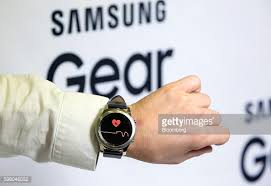
\includegraphics[scale=0.4]{images/gears3.jpg}
	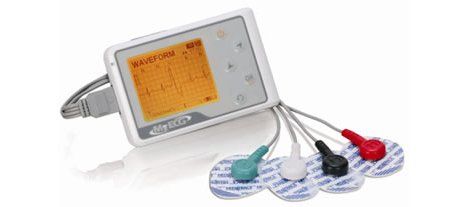
\includegraphics[scale=0.3]{images/ecg_1.jpg}	
	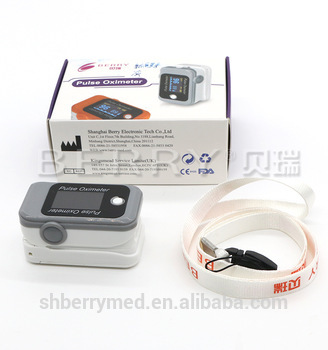
\includegraphics[scale=1]{images/ppg_clip.jpg}
	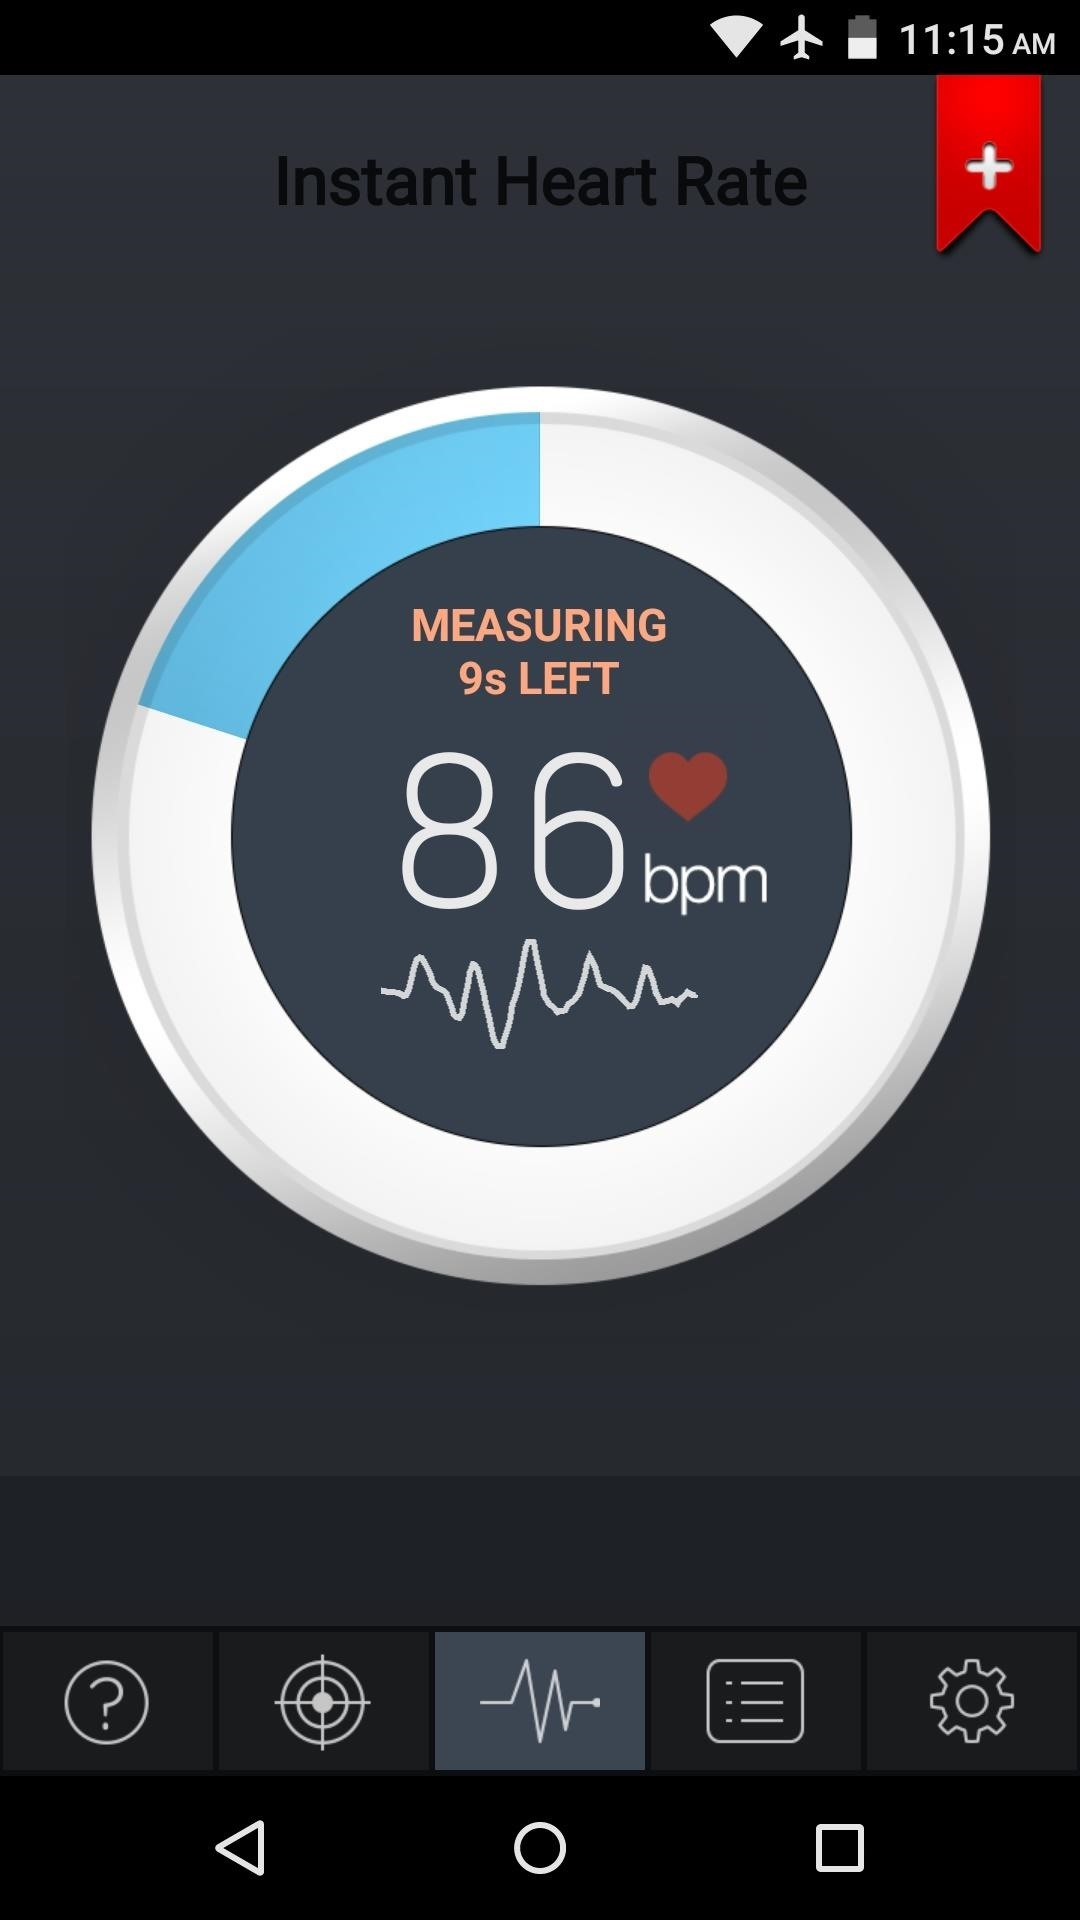
\includegraphics[scale=0.04]{images/heart_app1.jpg}
    \caption{a) Samsung Gear S3; b) Holter Monitor; c) Fingertip Pulse Oximeter; d) Heart Rate App}
    \label{fig:device_example}
\end{figure}

\begin{table}[H]
	\centering
	\begin{tabular}{|l|L{4cm}|c|L{0.5cm}|L{0.5cm}|L{0.5cm}|L{0.5cm}|L{0.5cm}|L{0.5cm}|L{0.5cm}|L{0.5cm}|}
		\hline
		\rowcolor{gray}
		\textbf{No} & \textbf{Aplikasi} & \textbf{Sen} & \multicolumn{8}{c}{\textbf{Fitur}} \\
		\rowcolor{gray}
		 & & \textbf{sor} & A & B & C & D & E & F & G & H \\
		\hline
		1 & Instant Heart Rate : Heart Rate \& Pulse Monitor & PPG & Y & N & Y & Y & N & Y & N & Y \\
		2 & iCare Health Monitor (BP \& HR) & PPG & Y & N & Y & N & N & Y & N & Y \\
		3 & Heart Rate Monitor(REPS) & PPG & Y & N & Y & Y & N & Y & N & Y \\
		4 & Runtastic Heart Rate Monitor \& Pulse Checker & PPG & Y & N & Y & N & N & Y & N & N \\
		5 & Cardiograph - Heart Rate Meter & PPG & Y & N & Y & Y & N & Y & N & Y \\
		6 & ASUS Heart Rate & PPG & N & N & N & N & N & Y & N & N \\
		7 & Samsung Health & PPG & Y & Y & N & N & N & Y & N & Y \\
		8 & Heart Rate Monitor(Meet Your Need Production) & PPG & N & N & N & N & N & Y & N & N \\
		9 & \textbf{MobECG} & \textbf{ECG} & N & Y & Y & Y & N & Y & N & N \\		
		10 & \textbf{CMS50Dplus} & \textbf{ECG} & N & Y & Y & Y & N & Y & N & N \\
		\hline
	\end{tabular}
	\caption{Perbandingan 10 Aplikasi Monitoring Jantung di Play Store}
	\label{table:app_comparison}
\end{table}

\begin{table}[H]
	\centering
	\begin{tabular}{|l|L{3cm}|c|c|c|L{0.5cm}|L{0.5cm}|L{0.5cm}|L{0.5cm}|L{0.5cm}|L{0.5cm}|L{0.5cm}|L{0.5cm}|}
		\hline
		\rowcolor{gray}
		\textbf{No} & \textbf{Produk} & \textbf{Sen} & \textbf{Me} & \textbf{Op} & \multicolumn{8}{c}{\textbf{Fitur}} \\
		\rowcolor{gray}
		 & & \textbf{sor} & \textbf{dis} & \textbf{en} & A & B & C & D & E & F & G & H \\
		\hline
		1 & Fitbit Blaze & PPG & N & N & Y & Y & Y & Y & N & Y & N & Y \\
		2 & Samsung Gear S3 & PPG & N & N & Y & Y & Y & N & N & Y & N & Y \\
		3 & ENDO SE-2003 & ECG & Y & N & Y & Y & Y & Y & N & Y & N & N \\
		4 & ENDO H-10 & PPG & Y & N & Y & Y & Y & Y & N & Y & N & N \\
		\hline
	\end{tabular}
	\caption{Perbandingan Produk Berupa Alat}
	\label{table:product_comparison}
\end{table}

Ket: \\
A = Identitas User \\
B = Real Time Monitoring \\
C = Melihat Gelombang Jantung \\
D = Merekam Gelombang Jantung \\
E = Multiuser Monitoring \\
F = Deteksi BPM \\
G = Aritmia Alert \\
H = Share Result via Network \\

\subsection{Riset Terkait}
Arsitektur sistem yang dirancang pada tugas akhir ini menerapkan konsep Internet of Things (IoT) dan diharapkan mampu melakukan analisis otomatis, khususnya aritmia. Penerapan IoT kedalam \textit{monitoring} jantung sudah pernah dilakukan sebelumnya, begitupun dengan analisis artimia secara otomatis. Untuk mengoptimalkan metode yang diajukan pada tugas akhir ini, diperlukan pembelajaran terhadap riset terkait atas kedua hal tersebut.

Pada tahun 2013, Daniel Barata dan rekannya dari Portugal merancang metode \textit{monitoring} yang dapat bekerja secara \textit{portable} \cite{daniel_barataa}. Sensor yang terhubung dengan sebuah tablet android akan berkomunikasi menggunakan protokol MQTT. Penggunaan MQTT memungkinkan \textit{throughtput} data yang besar dan banyak sensor yang terhubung secara bersamaan. Metode ini menggunakan sensor ECG dan PPG untuk mengambil data tubuh. Pemilihan MQTT untuk meningkatkan jumlah sensor yang dapat terhubung juga dilakukan oleh Karan Motwani pada penilitiannya di tahun 2016 \cite{karan_motwani}. Selain digunakan untuk \textit{monitoring} MQTT juga digunakan pada \textit{facebook messager} [].

Pada tahun 2014, Paola Pierleoni dan rekannya merancang metode monitoring yang melibatkan ponsel dan sensor ECG milik produk "Zephyr HxM-BT" \cite{paola_pierleoni}. Zephyr akan mengirimkan sinyal ECG melalui bluetooth menuju polsel untuk di proses. Metode \textit{monitoring} yang dirancang oleh Pierleoni menambahkan analisis aritmia kedalamnya. Aritmia dianalisis menggunakan \textit{rule based classification} yang diusulkan oleh Tsipouras(2005). Aturan yang diajukan oleh Tsipouras memerhatikan fitur RR interval dari gelombang jantung \cite{rr_classification}. Hasil analisis yang dihasilkan dapat dilihat secara \textit{real time} pada layar ponsel.

Pada tahun 2016, Vasu Jindal (seorang peneliti dari Universitas Texas) merancang metode \textit{monitoring} yang melibatkan penggunaan ponsel dan \textit{cloud}\cite{vasu_jindal}. Ponsel akan membaca gelombang jantung dari sensor PPG milik produk sejenis Fitbit, kemudian mengirimkannya ke \textit{cloud} untuk di proses. \textit{Cloud} akan memprosesnya menggunakan \textit{deep belief network} dan mengembalikan hasil pengukuran berupa BPM. Setiap data gelombang jantung yang diterima \textit{cloud} akan disimpan sebagai bahan prediksi berikutnya.

Di tempat lain pada tahun 2016, Mamidi Manisha dan rekannya dari India merancang metode \textit{monitoring} yang mirip dengan metode Jindal. Metode Mamidi juga melibatkan ponsel, produk jam tangan pintar \cite{mamidi} dan \textit{cloud processing}. Namun fokus utama dalam sistem yang mereka rancang ialah tentang bagaimana cloud dapat menangani pertukaran data yang besar dan cepat. Salah satu kunci keberhasilan sistem mereka ialah penerapan \textit{database} No-SQL yang berhasil memaksimalkan kecepatan penulisan data. Selain komunikasi yang cepat, sistem mereka dirancang agar memiliki mekanisme pemberitaan darurat kepada rumah sakit.

Dari keempat riset diatas, masing masing memiliki kelebihan dan kekurangan. Metode Lou dan Motwani dapat menghubungkan banyak sensor sekaligus. Metode Pierloeni dapat medeteksi aritmia tapi hanya pasien yang bisa mengetahuinya. Metode Jindal memiliki sistem analisis terpusat sehingga algoritma yang diterapkan dapat terus berkembang semakin akurat namun hanya bisa menganalisis BPM. Metode Manisha memiliki kehandalan dalam menangani banyak pasien dalam sistem terpusat dan mampu memberikan pemberitaan darurat namun analisis masih harus dilakukan manual. Ringkasan mengenai kelebihan dan kekurangan ini dapat dilihat pada tabel \ref{table:monitoring_compare}.

\begin{table}[H]
	\begin{tabular}{|L{5cm}|L{3cm}|C{1cm}|c|c|c|c|c|}
		\hline
		\rowcolor{gray}
		\textbf{Judul} & \textbf{Penulis} & \textbf{Ta} & \multicolumn{5}{c}{\textbf{Fitur}} \\
		\rowcolor{gray}
		 & & \textbf{hun} & A & B & C & D & E \\
		 An Android-Based Heart Monitoring System for the Elderly and
for Patients with Heart Disease & Paola Pierleoni, Luca Pernini, et al. & 2014 & Y & Y & N & N & Y \\
		\hline
		Integrating Mobile and Cloud for PPG Signal Selection to Monitor Heart Rate During Intensive Physical Exercise & Vasu Jindal & 2016 & Y & N & Y & N & N \\
		\hline
		IoT on Heart Attack Detection and Heart Rate Monitoring & Mamidi Manisha, Katakam Neeraja, et al. & 2016 & N & N & Y & Y & Y \\
		\hline
	\end{tabular}
	\caption{Perbandingan Riset Metode Monitoring}
	\label{table:monitoring_compare}
\end{table}

Ket: \\
A = Deteksi BPM \\
B = Deteksi Artimia \\
C = Sistem Deteksi Terpusat \\
D = Optimasi banyak pengguna \\
E = Sistem Peringatan \\

Pada konsep IoT, terdapat sedikitnya 3 komponen dalam aristekturnya yaitu \textit{sensor}, \textit{server} dan \textit{actuator}. \textit{Sensor} sebagai pengubah data dari dunia nyata ke bentuk digital agar dipahami oleh mesin. \textit{Server} sebagai pemroses data tersebut. Server

memberi Analisis terhadap rekam jantung Untuk mengklasifikasian aritmia seorang dokter perlu melihat hasil rekam jantung seorang pasien seperti gambar \ref{fig:contoh_aritmia}, baik hasil rekam ECG maupun PPG. Akan sangat melelahkan jika seorang dokter secara terus menerus memeriksa rekam jantung seorang pasien. Oleh karena itu dibutuhkan sebuah algoritma yang dapat melakukan klasifikasi secara otomatis. 

Telah banyak penelitian yang dilakukan yang melakukan otomasi klasifikasi aritmia[xx]. Kini penelitian tersebut telah memiliki keakuratan yang cukup baik, mencapai 90\%, dengan berbagai macam metode dan ekstraksi fitur.

Pada tahun xxx, asme asme asem

Pada tahun xxx, asme asme asem

Pada tahun xxx, asme asme asem

Pada tahun xxx, asme asme asem

Pada tahun xxx, asme asme asem

Pada tahun xxx, asme asme asem

\begin{table}[H]
\centering
	\begin{tabular}{|c|c|c|c|c|}
	\hline
	\rowcolor{gray}
	\textbf{Judul} & \textbf{Penulis} & \textbf{Fitur} & \textbf{Metode}  & \textbf{Hasil}\\
	\cline{1-5}
	Penemuan bla bla adu adu & Alif Akbar & Titik R & Decisin & 90\% \\
	\cline{1-5}
	Penemuan bla bla adu adu & Alif Akbar & Titik R & Decisin & 90\% \\
	\cline{1-5}
	Penemuan bla bla adu adu & Alif Akbar & Titik R & Decisin & 90\% \\
	\hline
	\end{tabular}
	\caption{Perbandingan riset mengenai klasifikasi aritmia otomasis}
	\label{table:research_comparison}
\end{table}

\section{ECG dan PPG}
Terdapat 2 jenis sensor yang umum digunakan untuk melakukan \textit{monitoring} jantung, yaitu \textit{Electrocardiogram} (ECG) dan \textit{Photoplethysmogram} (PPG) seperti yang terlihat pada gambar \ref{fig:ecg_n_ppg}. Kedua jenis sensor ini menjadi pilihan utama dalam \textit{monitoring} jantung karena keduanya mengusung konsep \textit{non-invasive}. Sensor non-invasive memungkinkan melakukan pengambilan data tubuh tanpa perlu melukai/menusuk bagian tubuh tertentu. Secara umum ECG akan menghasilkan pengukuran lebih akurat dari pada PPG. Namun PPG lebih nyaman digunakan dalam jangka panjang dari pada ECG.

\begin{figure}[H]
    \centering
    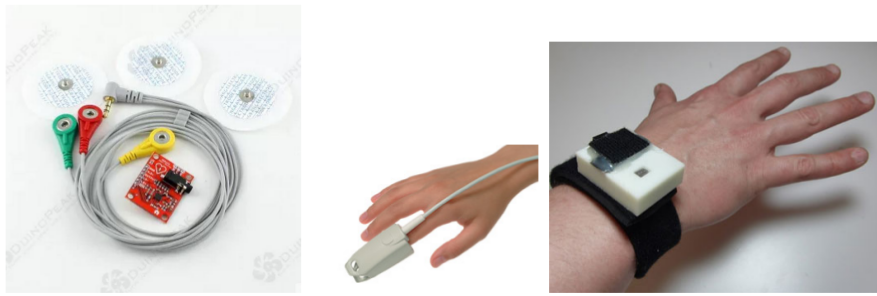
\includegraphics[scale=0.3]{images/sensors.png}
    \caption{a. Sensor ECG dengan 3 \textit{leads}; b. Sensor PPG ujung jari; c. Sensor PPG di pergelangan tangan}
    \label{fig:ecg_n_ppg}
\end{figure}

\subsection{Lokasi Penempatan Sensor}
\subsubsection{ECG}
ECG perlu melakukan pengukuran minimal di 3 lokasi. Hal ini disebabkan karena ECG secara langsung mengukur perubahan nilai kelistrikan yang dihasilkan tubuh. Untuk mengukur kelistrikan tubuh ECG memerlukan minimal 3 elektroda yaitu + (positif), - (negatif) dan N (netral), terlihat pada gambar \ref{fig:electrode3}. Untuk pengukuran lebih dari 3 titik, elektroda ECG dapat diletakkan pada posisi yang ditunjukkan gambar \ref{fig:multi_elctrode}.

\begin{figure}[H]
    \centering
    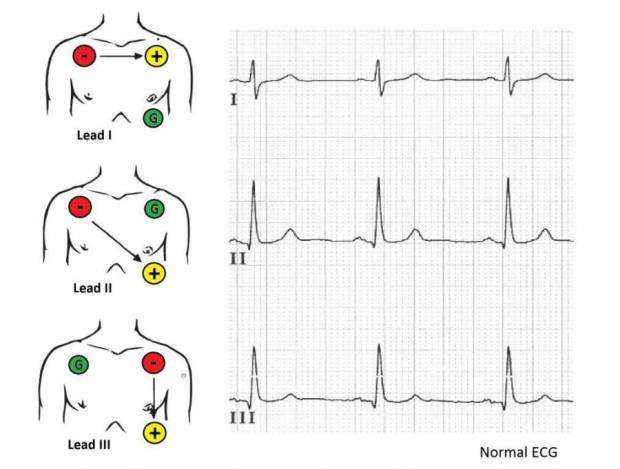
\includegraphics[scale=0.3]{images/3_ecg_place.jpg}
	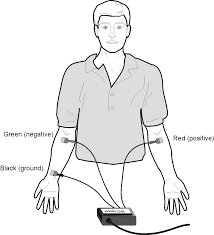
\includegraphics[scale=0.6]{images/3_ecg_place_2.png}    
    \caption{a. Penempatan 3 Elektroda di Dada, b. Penempatan 3 Elektroda di Tangan}
    \label{fig:electrode3}
	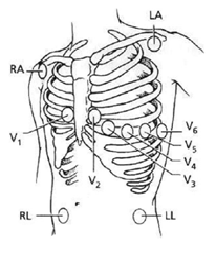
\includegraphics[scale=0.8]{images/multi_ecg.png}
    \caption{Lokasi Penempatan Lebih 3 titik}
    \label{fig:multi_elctrode}
\end{figure}

\subsubsection{PPG}
PPG dapat melakukan pengukuran hanya di satu lokasi. Hal ini disebabkan karena PPG mengukur tingkat penyerapan cahaya oleh darah, sedangkan pembuluh darah menjalar ke seluruh tubuh. Namun, untuk menghasilkan pengukuran maksimal PPG perlu diletakkan di lokasi tubuh yang pembuluh darah dekat dengan permukaan kulit \cite{ppg_placement}\cite{ppg_placement2}. Beberapa lokasi tubuh yang sesuai kriteria tersebut terdapat pada ujung jari, pergelangan tangan, lengan atas, leher, dan daun kuping.


\subsection{Titik Fiducial}
Untuk mengenali sebuah detak jatung pada rekam ECG maupun PPG diperlukan untuk mencari titik titik \textit{fiducial} (pembanding). Kemunculan titik fiducial menandakan adanya siklus \textit{beat} (detak) pada waktu kemunculan titik tersebut. Sebuah siklus sinyal ECG dapat dilihat dari beberapa titik fiducial yaitu P-QRS-T, seperti terlihat pada gambar \ref{fig:ecg_points}. Sedangkan siklus sinyal PPG dilihat dari siklus Diastolic-Systolic-Dicrotic seperti terlihat pada gambar \ref{fig:ppg_points}

\begin{figure}[H]
    \centering
    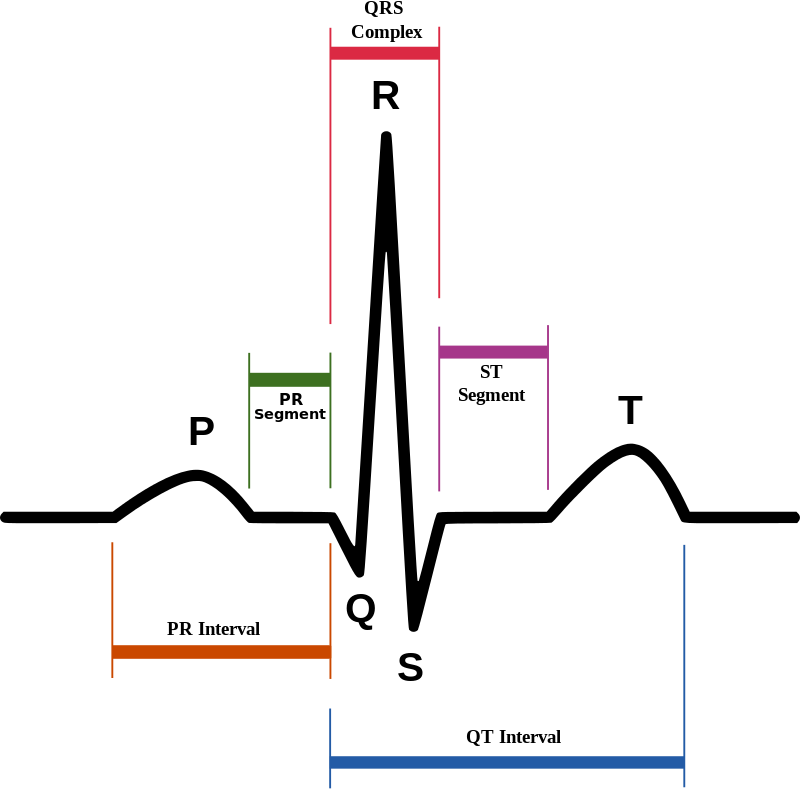
\includegraphics[scale=0.2]{images/ecg_points.png}
    \caption{Sinyal ECG berdasarkan titik fiducial}
    \label{fig:ecg_points}
	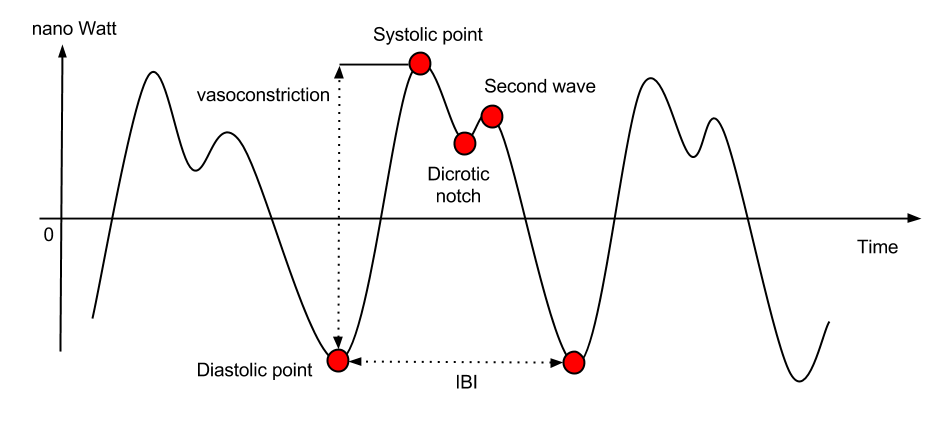
\includegraphics[scale=0.3]{images/PPG2.png}
    \caption{Sinyal PPG berdasarkan titik fiducial}
    \label{fig:ppg_points}
\end{figure}


\subsection{Bentuk Sinyal}
Dapat dilihat, pada gambar \ref{fig:ecg_vs_ppg}, dengan mudah bahwa sinyal bentukan dari PPG dengan ECG berbeda secara morfologi (bentuk)\cite{ppg_vs_ecg}. Namun, karena sumber sinyal yang sama (dari jantung) siklus PPG dan ECG dapat disinkronisasi (saling dipetakan) berdasarkan titik R pada ECG dan puncak sistolik pada PPG seperti gambar \ref{fig:ecg_vs_ppg2} \cite{ecg_syncro}. Perbedaan waktu kemunculan R dan Sistolik dikenal sebagai \textit{Pulse Arrival Time} (PAT). PAT dapat digunakan sebagai parameter mengukur tekanan darah, yang mana tidak dicakup pada tugas akhir ini.

\begin{figure}[H]
    \centering
    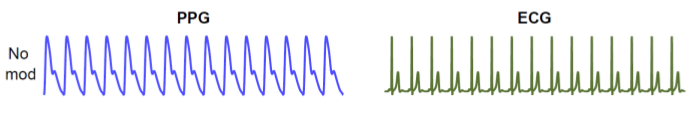
\includegraphics[scale=0.6]{images/ecg_vs_ppg.png}
    \caption{Perbandingan sinyal ideal PPG dan ECG}
    \label{fig:ecg_vs_ppg}
	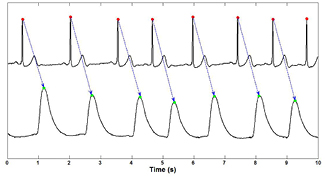
\includegraphics[scale=0.8]{images/sinkronisasi.jpg}
    \caption{Sinkronisasi antara ECG dan PPG}
    \label{fig:ecg_vs_ppg2}
\end{figure}

\section{Aritmia}
Aritmia adalah kategori gangguan jantung yang berupa tidak normal-nya irama jantung. Beberapa panyakit jantung yang tergolong aritmia antara lain:
\begin{itemize}
	\item \textit{Tachycardia} (detak lebih cepat dari normal),
	\item \textit{Bradycardia} (detak lebih lambat dari normal),
	\item \textit{Premature Atrial Contraction} (PAC),
	\item \textit{Premature Vantricular Contraction} (PVC),
	\item \textit{Ventricular Tachycardia} (VT) (detak ventrikel sangat cepat), dan
	\item \textit{Ventricular Fibrillation} (VF) (detak ventrikel tidak beraturan).
\end{itemize}

\textit{Premature Contraction} berarti siklus detak yang \textit{premature} (tidak pada waktunya) disebabkan oleh kontraksi pada atrium (bilik) atau ventrikel (serambi) terjadi lebih cepat atau lebih lambat dari seharusnya. \textit{Premature Contraction} tergolong serangan kecil (tidak berbahaya)[xx], sedangkan VT dan VF tergolong serangan besar (berbahaya). \textit{Premature contraction} yang terjadi berulang kali dan cepat merupakan awal dari peristiwa VT maupun VF. Contoh kemunculan PAC, PVC dan VF dapat dilihat pada gambar \ref{fig:contoh_aritmia}.

\begin{figure}[H]
    \centering
    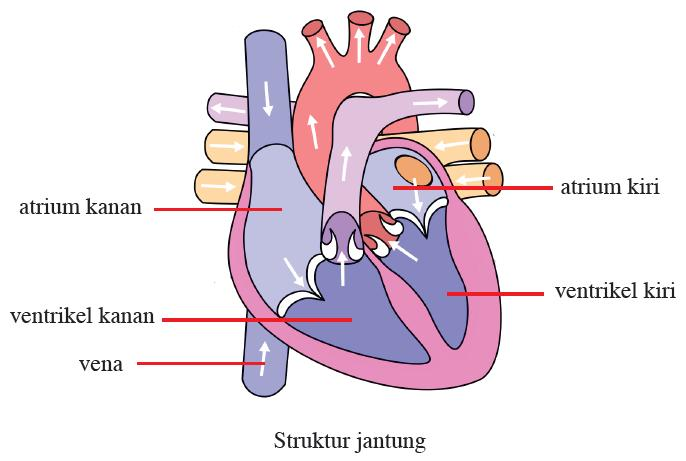
\includegraphics[scale=0.4]{images/jantung.jpg}
    \caption{Struktur jantung sederhana}
	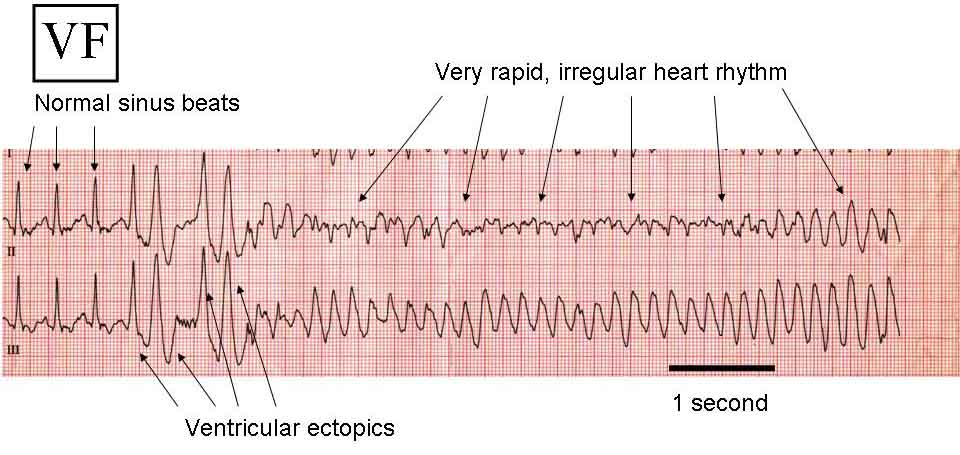
\includegraphics[scale=1.2]{images/VF.jpg}
    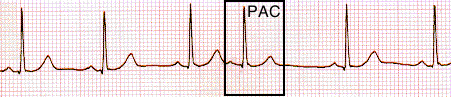
\includegraphics[scale=0.5]{images/PAC1.png}
	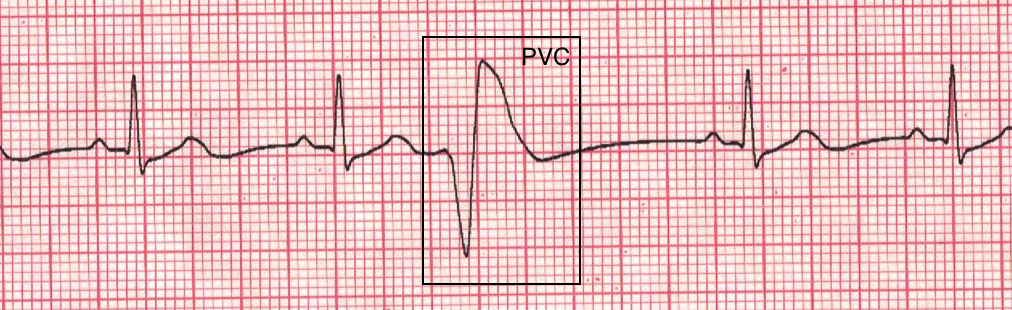
\includegraphics[scale=0.25]{images/PVC1.png}
    \caption{a. Sinyal VF; b. Sinyal PAC; c. Sinyal PVC}
    \label{fig:contoh_aritmia}	
\end{figure}


\section{Server dan Database}
%BARU
IoT memungkinkan komunikasi \textit{Machine to Machine} (M2M) terjadi dalam jaringan Internet. Hal ini berarti \textit{sensor}, \textit{server} dan \textit{receptor} berkomunikasi dimana saja selama dapat terhubung dengan Internet. Selain itu, IoT memodelkan agar banyak objek (\textit{Things}) dapat saling berkomunikasi. Sehingga, sebuah sistem yang dirancang untuk menangani banyak objek saling berkomunikasi dimana saja perlu menerapkan IoT.

Sebuah sistem monitoring yang dapat berjalan secara Ubiquitous haruslah dibangun dengan konsep \textit{Internet of Things} (IoT). IoT ialah konsep dimana objek objek (Things) dapat saling berinteraksi pada jaringan Internet tanpa membutuhkan manusia. Pada konsep IoT diperlukan setidaknya 3 komponen yaitu Sensor, Server dan Actuator. Sensor berfungsi sebagai pengambil data. Server yang menjalankan \textit{web service} (layanan web, contoh: http server, mqtt broker dan db server) berfungsi sebagai pengolah data. Actuator berfungsi sebagai pelaksana perintah dari server, seperti mengeluarkan suara dan membelokkan/memutus arus listrik. Node.Js dan Mongo.Db, keduanya dibutuhkan untuk membangun sebuah web service pada server.

\subsection{Node.Js}
Node.Js adalah teknologi Javascript (Js) \textit{Runtime} yang dibangun diatas Chrome V8 JS Engine. Node.Js memungkinkan bahasa pemrograman Js menjalankan web service. Node.Js dirancang menggunakan skema \textit{event-driven} dan \textit{non-blocking IO}, sangat sesuai untuk aplikasi \textit{data-intensive real-time} \cite{nodejs}. Node.JS juga telah terbukti secara performansi lebih cepat dari bahasa scripting lain seperti PHP, Python, dan Ruby bahkan tidak jauh lambat dibanding bahasa ter-\textit{compile} seperti JAVA, C, dan C++ \cite{node_comparisson}.

\subsection{MongoDB}
MongoDB adalah salah satu jenis program penyimpanan data yang bersifat NoSQL. MongoDB menyimpan data dengan bentuk dokumen dan format JSON. MongoDB dirancang untuk kasus penggunaan yang \cite{why_mongo}:
\begin{enumerate}
	\item Membutuhkan beban penulisan data yang tinggi,
	\item Skema data yang tidak stabil,
	\item Ukuran data akan menjadi sangat besar,
	\item Tidak memiliki seorang \textit{administrator}
\end{enumerate}

\begin{figure}[H]
    \centering
	
\includegraphics[scale=0.15]{images/nodejs.png}
    
\includegraphics[scale=0.3]{images/mongodb.png}
    \caption{a. Node JS; b. Mongo DB;}
\end{figure}

\section{ESP-12}
ESP-12 adalah salah satu tipe \textit{System on Module} (SoC) yang diproduksi oleh Espressif dari China. SoC berarti papan sirkuit yang telah terintegrasi oleh sistem tertentu. Kelebihan utama ESP ialah ukurannya yang kecil (16x24x3 mm) tapi dapat berfungsi sebagai \textit{controller} dan telah dilengkapi modul Wi-Fi. Hal ini memungkinkan komunikasi sensor-server melalui jaringan WiFi tanpa perlu menambah modul jaringan lagi.

\begin{figure}[H]
	\centering
	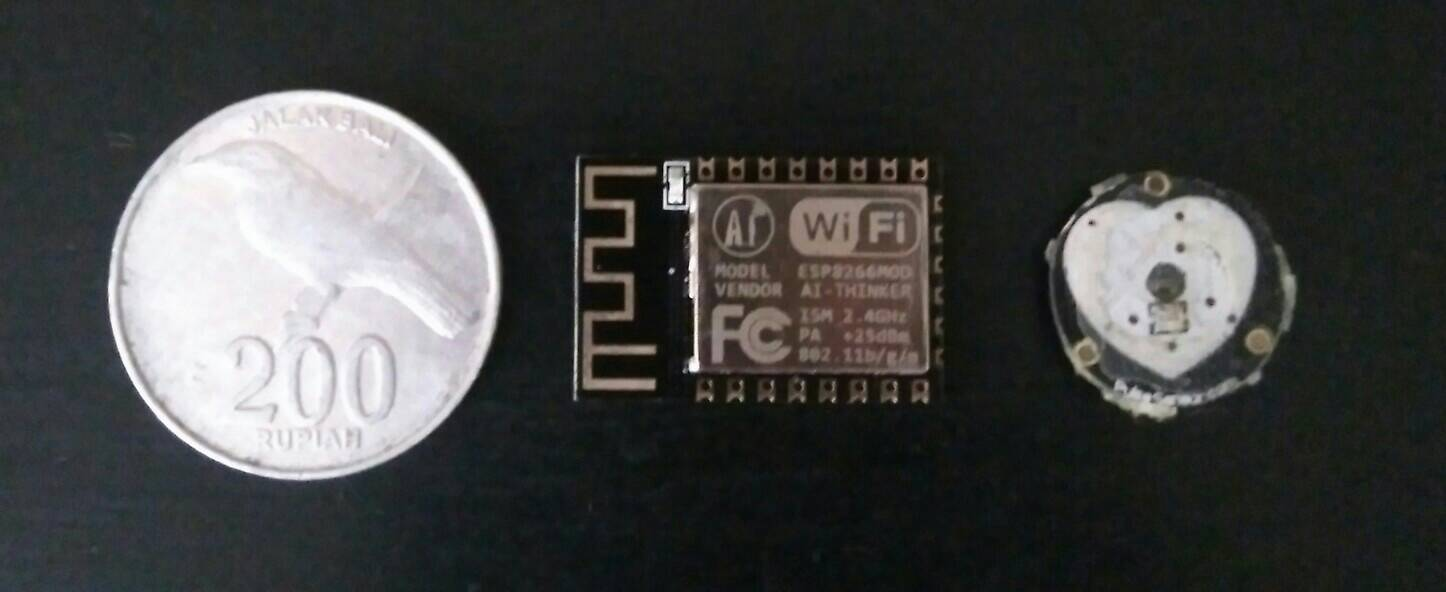
\includegraphics[scale=0.22]{images/coin_esp_pulse.jpg}
	\caption{Koin Rp200 - ESP-12E - Pulse Sensor}
	\label{fig:coin_esp_pulse}
\end{figure}

\section{Protokol MQTT}
Message Queuing Telemetry Transport (MQTT) adalah protokol transport
dengan skema komunikasi publish dan subscribe. MQTT dirancang menjadi protokol yang ringan, terbuka dan sederhana. Karakteristik ini membuat MQTT sangat tepat untuk digunakan sebagai protokol komunikasi machine-to-machine (M2M) dan Internet of Things (IoT). Protokol ini menggunakan TCP/IP pada layer transport. Terdapat tiga level Qualities of Service (QoS) dalam penyampaian pesan yaitu:
\begin{enumerate}
	\item QOS 0 atau “At most once”, dimana pesan dikirim dengan skema \textit{fire-and-forget} yang berarti tidak ada upaya menjamin pesan yang dikirim dapat sampai ke tujuan.
	\item QOS 1 atau “At least once”, dimana pesan dikirim dengan jaminan setidaknya pesan sampai sekali ke tujuan. Sehingga memungkinkan terjadinya duplikasi pesan di tujuan akibat pesan yang dikirim ulang dari pengirim.
	\item QOS 2 atau "Exactly once", dimana pesan dikirm dengan jaminan diterima tepat sekali ke tujuan. Sehingga tidak ada pesan yang terduplikasi di tujuan.	
\end{enumerate}

\begin{figure}[H]
	\centering
	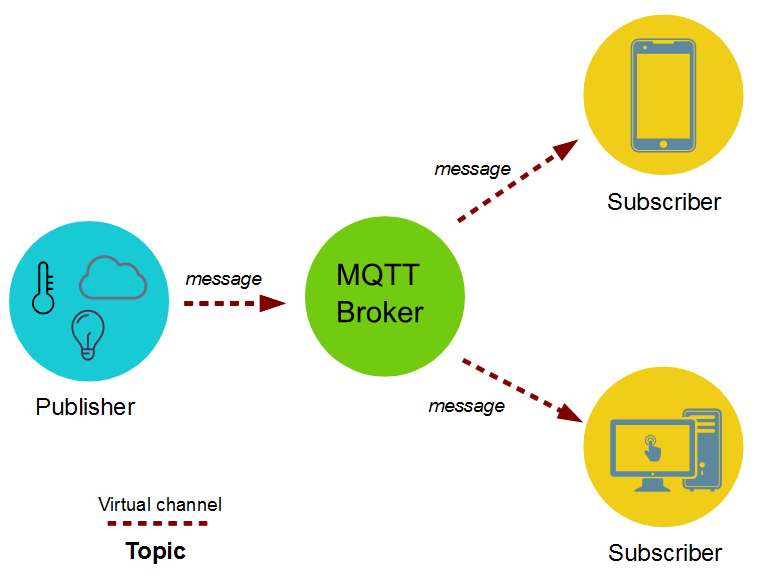
\includegraphics[scale=0.45]{images/mqtt.png}
	\caption{Cara kerja MQTT}
\end{figure}


%
\chapter{Metodologi dan Desain Sistem}
%\subsection{Flowchart Metodologi}
%Definisikan bentuk dan warna

\usetikzlibrary{positioning}
\tikzstyle{cloud} = [draw, ellipse, minimum height=2em]
\tikzstyle{io} = [trapezium, trapezium left angle=70, trapezium right angle=110, minimum width=3cm, minimum height=1cm, text centered, draw=black]
\tikzstyle{process} = [rectangle, minimum width=3cm, minimum height=1cm, text centered, minimum width=3cm, draw=black]
\tikzstyle{decision} = [diamond, minimum width=3cm, minimum height=1cm, text centered, draw=black]
\tikzstyle{arrow} = [thick,->,>=stealth]

\section{Metodologi Penelitian}
Diagram alir metodologi yang digunakan untuk menyelesaikan tugas akhir ditampilkan pada gambar \ref{flow:fig_flow_method}. Berikut penjelasan tiap tahap pada diagram alir tersebut:

\begin{figure}[H]
    \centering
	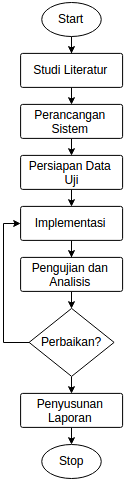
\includegraphics[scale=0.73]{images/flowchart_metodologi.png}
    \caption{Flowchart Metodologi}
	\label{flow:fig_flow_method}
\end{figure}

\begin{enumerate}
	\item \textbf{Studi literatur} \\
	Pada tahap ini penulis mengumpulkan literatur seperti buku, artikel dan \textit{paper} yang berguna menjadi landasan informasi pada penelitian. Hasil tahap ini ialah fakta dan teori serta masalah yang dihadapi.
	\item \textbf{Perancangan Sistem} \\
	Pada tahap ini penulis memilah masalah yang dapat diselesaikan berdasarkan fakta dan teori yang telah dikumpulkan. Hasil tahap ini ialah rancangan sistem yang diajukan sebagai solusi.
	\item \textbf{Persiapan Data Uji} \\
	Pada tahap ini penulis mempersiapkan data yang telah tervalidasi kebenarannya untuk dijadikan input pengujian. Hasil tahap ini ialah dataset yang telah dianotasi.
	\item \textbf{Implementasi} \\
	Pada tahap ini penulis menerapkan rancangan sistem baik yang berupa \textit{software} maupun \textit{hardware}. Hasil tahap ini ialah \textit{software} dan \textit{hardware} yang dapat berjalan tanpa masalah.
	\item \textbf{Pengujian dan Analisis} \\
	Pada tahap ini penulis melakukan pengujian terhadap sistem yang dibangun menggunakan data uji dan parameter pengujian. Jika ditemukan ada masalah teknis ataupun kemungkinan melakukan peningkatan performansi maka penulis akan kembali ke tahap implementasi. Hasil tahap ini ialah \textit{software} dan \textit{hardware} dengan konfigurasi terbaik yang ditemukan.
	\item \textbf{Penyusunan Laporan} \\
	Pada tahap ini penulis melakukan penulisan laporan hasil akhir dari tugas akhir. Hasil dari tahap ini berupa buku tugas akhir dan jurnal penelitian.
\end{enumerate}

\section{Gambaran Umum Sistem}
Untuk menyelesaikan masalah yang ditemukan, penulis merancang sebuah solusi sistem untuk pemantauan jantung. Sistem dirancang untuk bisa dipantau di halaman \textit{web} dan ponsel android. Hasil kalkulasi sistem bukanlah analisa medis, tetapi hanya berupa peringatan. Analisis dokter masih diperlukan untuk mengambil keputusan medis terhadap peringatan yang diberikan oleh sistem. Pengguna sistem ialah dokter, pasien (pengguna yang memakai sensor), dan keluarga pasien. Sistem ditujukan untuk penggunaan non-medis atau sehari-hari yang berfungsi sebagai peringatan dini. Tujuan dari peringatan ini ialah:
\begin{enumerate}
	\item bagi pasien atau keluarga pasien agar mereka dapat menghubungi dokter untuk melakukan pengecekan lebih lanjut.
	\item bagi dokter agar dia dapat merancang pengobatan sesuai analis dokter tersebut.
\end{enumerate}

Secara umum sistem bekerja dimulai dari pengambilan data jantung menggunakan \textit{Receptor} yang diletakkan pada pergelangan tangan. Receptor kemudian secara periodik melakukan sampel dan mengirimkan sampel tersebut ke server untuk diproses lebih lanjut. Pengguna sistem dapat kapan saja melihat data aktivitas jantung melalui \textit{dashboard} berupa halaman \textit{web} atau ponsel android. Ketika server mendeteksi kemunculan artimia, server akan secara otomatis mengirimkan pesan peringatan kepada \textit{dashboard} di pengguna sistem. Arsitektur sistem secara umum digambarkan pada gambar \ref{fig:gambar_umum}.

\begin{figure}[H]
	\centering
	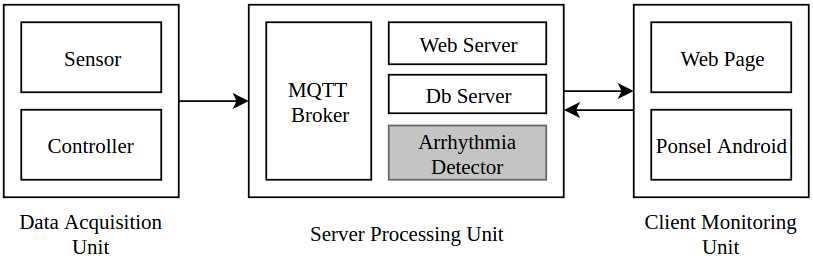
\includegraphics[scale=0.8]{images/gambar_umum.png}
    \caption{Gambaran Umum Sistem}
	\label{fig:gambar_umum}
\end{figure}

\section{Rancangan Perangkat Keras}
Sistem yang dirancang haruslah diimplementasikan untuk diuji coba. Oleh karena itu perlu dilakukan pemilihan perangkat keras. Perangkat keras dipilih berdasarkan pada kebutuhan rancangan sistem. Perangkat keras dibagi menjadi 3 bagian yaitu \textit{Receptor}, \textit{Server}, dan \textit{dashboard}.

Setelah perangkat keras ditentukan, algoritma yang sesuai untuk diterapkan harus dirancang. Rancangan algoritma terbagi menjadi 2 alur yaitu alur deteksi dan alur pemantauan. Rancangan algoritma dijelaskan lebih lengkap pada sub bab \ref{ssec:algorithm_design_1} dan sub bab \ref{ssec:algorithm_design_2}.

\subsection{Receptor}
Receptor berfungsi untuk mengambil data aktivitas jantung seorang pasien. Sistem yang dibangun tidak dapat menggunakan produk monitoring yang sudah ada karena sistem tersebut tidak bersifat \textit{Open Source}. Hal ini mengakibatkan penulis tidak bisa melakukan konfigurasi terhadap sensor dan \textit{controller}-nya. Konfigurasi yang dimaksud ialah menaikkan atau menurunkan frekuensi sampel dan transmit. Oleh karena itu penulis merancang receptor khusus untuk penelitian tugas akhir ini. Receptor dibangun dengan 3 komponen utama yaitu \textit{Sensor}, \textit{Controller}, dan baterai. Secara lengkap skema elektronik dapat dilihat pada gambar \ref{fig:schematics}.

\begin{figure}[H]
\centering
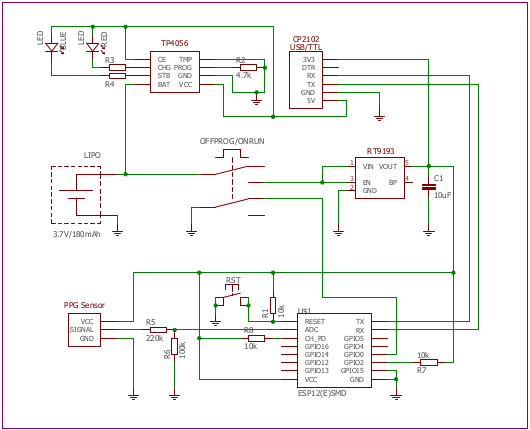
\includegraphics[scale=0.7]{images/schematics.png}
\caption{Skema Elektronik Receptor}
\label{fig:schematics}
\end{figure}

\subsubsection{a. Sensor}
Sistem dirancang untuk mengembangkan produk pemantauan jantung yang sudah ada di pasaran. Berdasarkan pengetahuan yang telah dibangun pada bab kajian pustaka, terdapat 2 jenis sensor yang umum digunakan yaitu ECG dan PPG. Berdasarkan rancangan algoritma pada sub bab \ref{ssec:algorithm_design} fitur yang dipilih dapat dihasilkan baik oleh ECG maupun PPG. Dengan demikian ECG dan PPG dapat digunakan dalam sistem.

Dalam tugas akhir ini, penulis memilih menggunakan PPG. Sensor PPG yang digunakan merupakan produksi Pulse Sensor yang dirancang oleh Joel dan Yury \cite{pulse_sensor}, terlihat pada gambar \ref{fig:coin_esp_pulse}. Alasan penulis milihan PPG ialah karena:
\begin{enumerate}
	\item harganya yang murah,
	\item PPG hanya menempel di satu bagian tubuh,
	\item PPG berukuran relatif kecil,
	\item kekurangan PPG yaitu kurang akurat dibanding ECG, tidak menyalahi tujuan sistem sebagai peringatan dini bukan medis.
\end{enumerate}

\subsubsection{b. Controller}
Sistem dirancang untuk monitoring terus menerus dan \textit{Ubiquitous}. Maka receptor haruslah cukup kecil untuk dibawa kemana saja dan menggunakan media komunikasi \textit{wireless} (tanpa kabel) untuk beriteraksi dengan server. Terdapat banyak jenis media komunikasi \textit{wireless} seperti GSM/CDMA, WiFi, Bluetooth, Infra Red, Zigbee, dll. WiFi dipilih sebagai media, pada sistem, karena jarak cakup yang cukup besar dan mudah untuk dikonfigurasi. Berdasarkan pengetahuan yang telah dibangun pada bab kajian pustaka, terdapat sebuah SoC yang telah memiliki kemampuan \textit{controller} dan memiliki modul WiFi dengan ukuran yang kecil yaitu ESP-12. Oleh karena itu receptor dirancang menggunakan ESP-12.

\subsubsection{c. Baterai}
Untuk memungkinkan receptor dibawa kemana saja dan dikenakan terus menerus diperlukan baterai sebagai catuan. Pada tugas akhir ini penulis menggunakan baterai \textit{Li-Polymer} (LiPo) \textit{protected} berkapasitas 180mAh dan tegangan 3.7V. Baterai ini juga berukuran kecil yaitu 25x18x8 mm dan memiliki bobot 5.3 gr, terlihat pada gambar \ref{fig:battery}.

\begin{figure}[H]
	\centering
	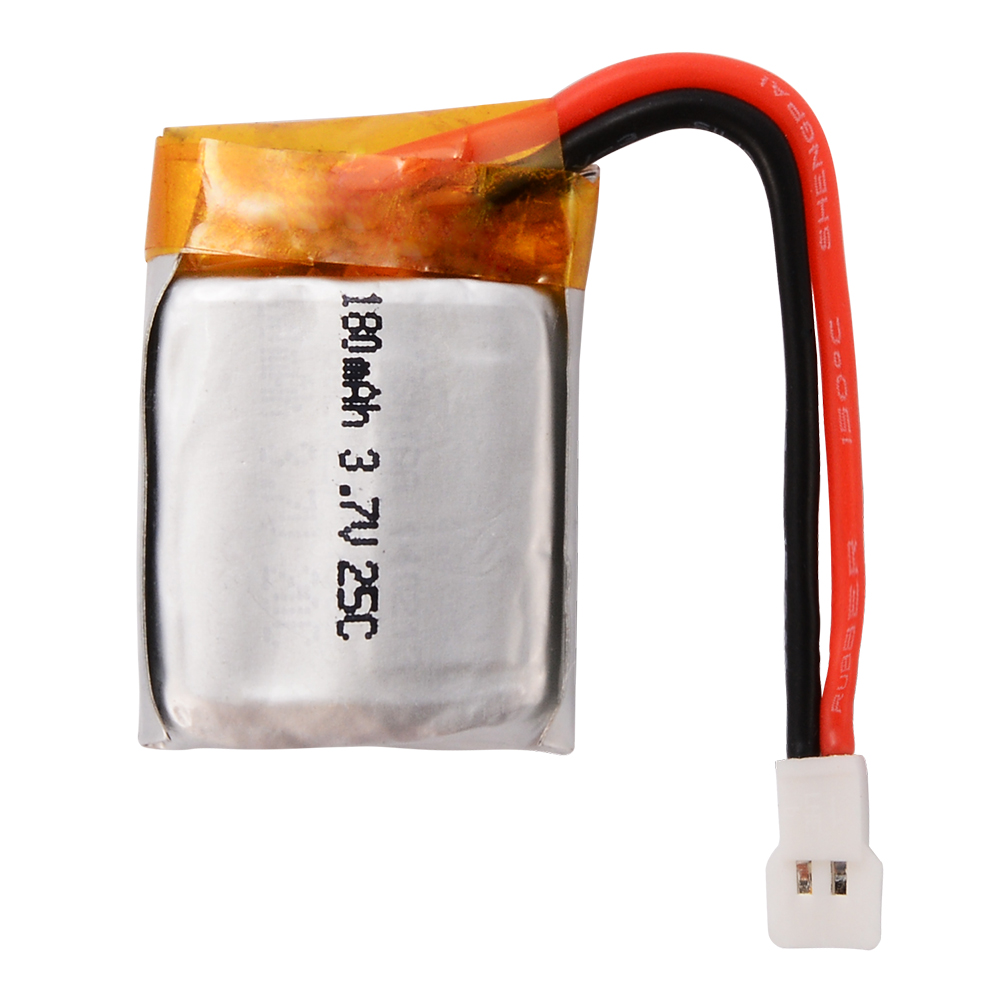
\includegraphics[scale=0.14]{images/baterai.jpg}
	\caption{Baterai LiPo 3.7v 180mAh}
	\label{fig:battery}
\end{figure}

\subsection{Server}
Untuk mengimplemantasikan konsep IoT server dirancang agar bisa melayani banyak \textit{receiver} dan \textit{dashboard}. Oleh karena itu server harus melayani komunikasi dengan arus data yang tinggi. Alasan ini mendorong penulis memilih menggunakan protokol MQTT sebagai protokol komunikasi, NodeJs sebagai runtime dan MongoDb sebagai penyimpanan data. Server dirancang agar bisa berjalan pada satu perangkat. Hal ini berarti MQTT broker, Web server, DB server, dan Algoritma Detector berjalan pada satu alamat IP yang sama. 

\subsection{Dashboard}
Sistem dirancang memiliki 2 saluran pemantauan yaitu halaman \textit{web} dan aplikasi pada ponsel Android. Kedua saluran ini dapat melakukan pemantauan selama berada dalam jaringan yang sama dengan server. Penulis memilih Android karena memiliki jumlah pengguna terbesar didunia[xx] sehingga bisa diasumsikan sistem yang dirancang bisa digunakan oleh banyak orang.

\subsubsection{a. Halaman Web}
Halaman web dibangun menggunakan \textit{framework} Express.Js. Pada halaman web terjadinya aritmia ditandai dengan bunyi dan bertambahnya angka hitungan aritmia yang terdeteksi. Tampilan halaman web dapat dilihat pada gambar \ref{fig:dashboard_apps}.

\subsubsection{b. Aplikasi Ponsel Android}
Aplikasi ponsel android dibangun untuk dapat berjalan pada ponsel android ber-OS (\textit{operating system}) minimal Jelly Bean (Android v4.1). Pada aplikasi ini terjadinya aritmia ditandai dengan bunyi atau berubahnya status deteksi dan kode warna ikon seru. Kode warna merah berarti terdeteksi aritmia berbahaya, kuning terdeteksi aritmia tidak berbahaya, dan hijau berarti kondisi normal. Tampilan aplikasi android dapat dilihat pada gambar \ref{fig:dashboard_apps}.

\begin{figure}[H]
	\centering
	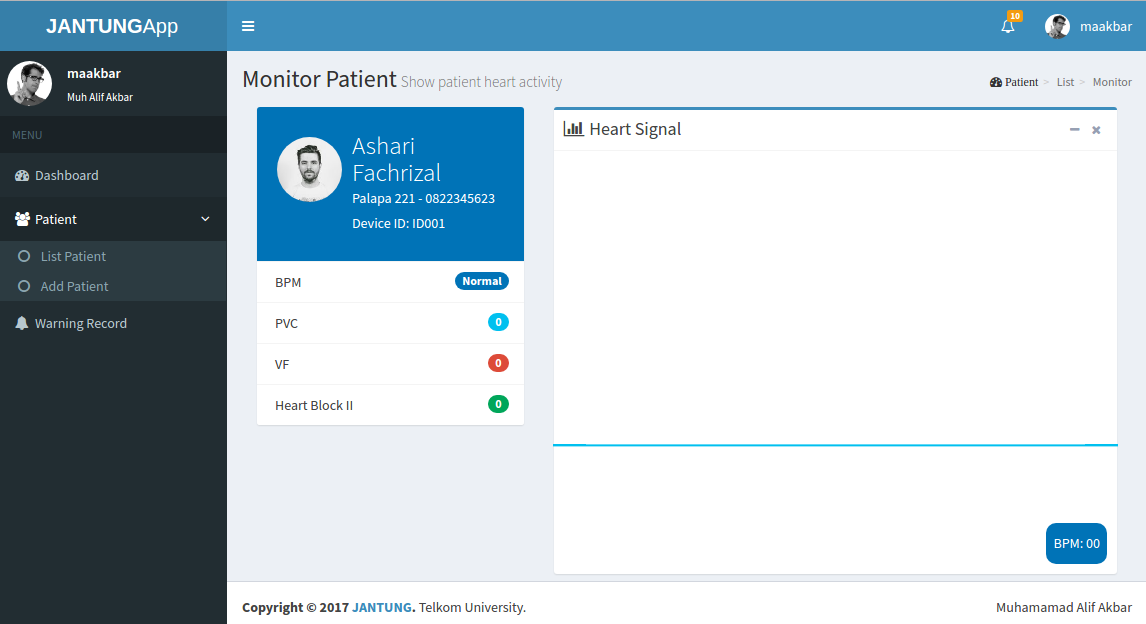
\includegraphics[scale=0.26]{images/web_app.png}
	\label{fig:dashboard_apps}
	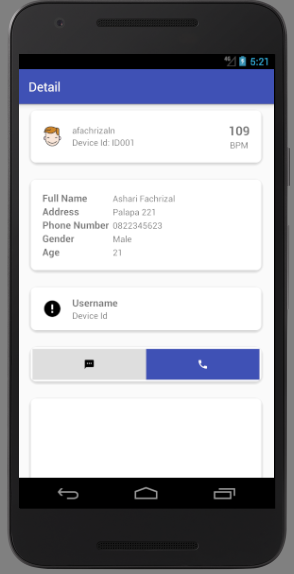
\includegraphics[scale=0.3]{images/phone_app.png}
	\caption{a) Tampilan Web Monitoring b) Tampilan Aplikasi Monitoring}
	\label{fig:dashboard_apps}
\end{figure}

\section{Rancangan Proses Pemantauan} \label{ssec:algorithm_design_1}
Fungsi utama dari sistem yang dibuat ialah melakukan pemantauan. Untuk melakukan pemantauan sistem perlu mengaplikasikan algoritma pemantauan. Algoritma pemantauan hanya berjalan pada perangkat \textit{dashboard} yaitu halaman \textit{web} atau aplikasi ponsel android. Diagram alir algoritma pemantauan dapat dilihat pada gambar \ref{flow:fig_report_algorithm}.
\begin{figure}[H]
	\centering
    %Mulai menggambar Flowchart
\begin{tikzpicture}[node distance=2cm]
\node (start) [cloud] {Start};
\node (open) [process, below of=start] {Membuka dashboard};
\node (input) [io, below of=open] {Memasukkan Kode Sensor / User};
\node (page) [process, below of=input] {Membuka Halaman Pemantauan};
\node (analysis) [process, below of=page] {Melakukan Analisis};
\node (stop) [cloud, below of=analysis] {Stop};
\draw [arrow] (start) -- (open);
\draw [arrow] (open) -- (input);
\draw [arrow] (input) -- (page);
\draw [arrow] (page) -- (analysis);
\draw [arrow] (analysis) -- (stop);
\end{tikzpicture}
    \caption{Flowchart Rancangan Algoritma Pemantauan}
	\label{flow:fig_report_algorithm}
\end{figure}

\textit{Flowchart} diatas (gambar \ref{flow:fig_report_algorithm}) dimulai dengan seorang pengguna baik pasien, keluarga pasien, maupun dokter perlu membuka sebuah perangkat \textit{dashboard}. Setelah aplikasi terbuka, baik web maupun aplikasi ponsel, user perlu memasukkan kode sensor atau user yang ingin dipantau. Setelah kode pantau dimasukkan aplikasi akan membuka halaman pemantauan. Setelah grafik pemantauan mulai berjalan pengguna bisa melakukan analisis.

\section{Rancangan Proses Deteksi} \label{ssec:algorithm_design_2}
Fungsi berikutnya yang akan diterapkan dalam sistem ialah dapat melakukan pendeteksian aritmia otomatis. Untuk itu sistem perlu menerapkan algoritma deteksi. Algoritma deteksi yang diterapkan pada tugas akhir ini terbagi menjadi 5 tahap yaitu Pengambilan dan Pengiriman Sinyal, Preprocessing dan Perekaman, Deteksi Detak Otomatis, Deteksi Aritmia Otomatis dan Pengiriman Laporan. Diagram alir tahap algoritma deteksi digambarkan pada gambar \ref{flow:fig_detect_algorithm}.

\begin{figure}[H]
	\centering
    %Mulai menggambar Flowchart
\begin{tikzpicture}[node distance=2cm]
\node (start) [cloud] {Start};
\node (get) [process, below of=start] {1. Pengambilan dan Pengiriman Sinyal};
\node (record) [process, below of=get] {2. Preprocessing dan Perekaman};
\node (beat) [process, below of=record] {3. Deteksi Detak Otomatis};
\node (aritmia) [process, below of=beat] {4. Deteksi Aritmia Otomatis};
\node (detected) [decision, below of=aritmia] {Terdeteksi?};
\node (report) [process, below of=detected] {5. Pengiriman Laporan};
\node (stop) [cloud, below of=report] {Stop};
\draw [arrow] (start) -- (get);
\draw [arrow] (get) -- (record);
\draw [arrow] (record) -- (beat);
\draw [arrow] (beat) -- (aritmia);
\draw [arrow] (aritmia) -- (detected);
\draw [arrow] (detected) -- (report);
\draw [arrow] (detected) -- ++(-80pt,0pt) |- (stop);
\draw [arrow] (report) -- (stop);
\end{tikzpicture}
    \caption{Flowchart Rancangan Algoritma Deteksi}
	\label{flow:fig_detect_algorithm}
\end{figure}

\subsection{Pengambilan dan Pengiriman Sinyal}
Pengambilan dan Pengiriman sinyal dilakukan di Receptor. Langkah pertama ialah \textit{controller} mengambil nilai pada pin analognya. Nilai pada pin analog lalu dikonversi menjadi satuan \textit{Volt}. Nilai yang telah dikonversi kemudian disisipkan header lalu dikirim  menggunakan protokol MQTT dengan QoS 0. \textit{Controller} kemudian tidur selama 2 ms lalu mengulang pengambilan dan pengiriman. Header berisi kode sensor dan angka index untuk menandakan urutan hasil bacaan. Index terebut direset setiap angka 1000. Diagram alir untuk memperjelas algoritma bagian ini dapat dilihat pada gambar \ref{flow:flow_sample}.

\begin{figure}[H]
\centering
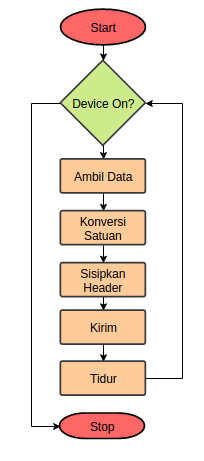
\includegraphics[scale=0.8]{images/flow_sample.png}
\caption{Flowchart Pengambilan dan Pengiriman Sinyal}
\label{flow:flow_sample}
\end{figure}

\subsection{Preprocessing dan Perekaman}
Setelah data diterima oleh server. Server melakukan \textit{preprocessing} pada data. \textit{Preprocessing} yang dilakukan terbagi menjadi \textit{data completer}, \textit{filtering}, \textit{squaring}, \textit{moving window integration}(MWI) dan \textit{Adaptive Thresholding}. Setelah \textit{filtering} dilakukan nilai dianggap telah bersih \textit{noise} maka nilai ini di simpan/rekam di \textit{database}. Preprocessing berlanjut ke \textit{squaring} dan MWI. Terakhir ekstraksi fitur \textit{peak} (R pada ECG dan Systolic pada PPG) dilakukan dengan \textit{Adaptive Thresholding}. Diagram alir algoritma \textit{preprocessing} dapat dilihat pada gambar \ref{flow:fig_preproc_algorithm}. Rangkaian \textit{preprocessing} ini merupakan modifikasi pada algoritma yang diusulkan oleh Pan-Tomkin (1985) (sub bab \ref{bab2_pantom}) dan Kalidas-Tamil (2016) agar kedua algoritma ini bisa bekerja untuk ECG dan PPG.

\subsubsection{a. Data Completer}
Data Completion berfungsi ialah algoritma untuk menangani hilangnya data selama pengiriman. Hal ini mungkin terjadi karena data dikirimkan dari \textit{receptor} menggunakan QoS 0. Pertama, data dipisahkan antara nilai pembacaan sensor dan header. Header kemudian digunakan untuk memisahkan proses perhitungan, setiap kode sensor akan memiliki proses sendiri. Jika terdapat locatan index pada header (index data yg diterima bukan bertambah 1 dari index data sebelumnya) maka proses akan menambah data buffer sebanyak jumlah index yang terlompati dengan nilai berdasarkan proyeksi garis lurus dari nilai terakhir ke nilai terbaru mengikuti persamaan \ref{eq:line}. Jika tidak ada nilai yang hilang maka nilai akan langsung dimasukkan ke buffer.

\begin{equation}
y(n) = \dfrac{n (y_{2} - y_{1})}{d} + v_{1}
\label{eq:line}
\end{equation}

$v_{1}$ adalah nilai terakhir yang diterima, $v_{2}$ adalah nilai terbaru yang diterima, $n$ adalah jarak dari index terakhir, $d$ adalah jarak index terbaru ke terakhir. $y$ adalah nilai index $n$ yang hilang

\subsubsection{b. Filtering}
Filtering berfungsi untuk menghilangkan noise yang mempengaruhi sinyal. \textit{Noise} yang umum terdapat ialah \textit{muscle noise} dan \textit{baseline wander}. Filtering yang diterapkan terbagi menjadi dua tahap yaitu \textit{Band Pass Finite Impulse Response(FIR) Filter} kemudian \textit{First Order Derivation Filter}. Tahap ini sesuai dangan algoritma yang diusulkan oleh Pan-Tomkins (1985)\cite{pantom} dan Kalidas-Tamil (2016) \cite{ecg_syncro}. \textit{Band Pass Filter} yang digunakan memiliki frekuensi response 5-15Hz. Daftar koefisien lengkap untuk \textit{Band Pass Filter} dan \textit{Derivation Filter} tercantum pada tabel x.x di bab lampiran.

\subsubsection{c. Squaring dan Moving Window Integration (MWI)}
Sesuai namanya \textit{Squaring} melakukan penguadratan (persamaan \ref{eq:square}) terhadap data. Sedangkan MWI melakukan penghalusan data berdasarkan n data sebelum. MWI dilakukan dengan persamaan \ref{eq:mwi}.

\begin{equation}
y = x^{2}
\label{eq:square}
\end{equation}
\begin{equation}
y(n) = 2v_{n} + v_{n-1} - v_{n-3} - 2v_{n-4}
\label{eq:mwi}
\end{equation}

\begin{figure}[H]
	\centering
    %Mulai menggambar Flowchart
\begin{tikzpicture}[node distance=2cm]
\node (start) [cloud] {Start};
\node (get) [io, below of=start] {Input Data Jantung};
\node (band) [process, below of=get] {Band Pass Filter};
\node (derr) [process, below of=band] {Derivation Filter};
\node (save) [process, below of=derr] {Simpan Hasil};
\node (square) [process, below of=save] {Squaring};
\node (mwi) [process, below of=square] {MWI};
\node (stop) [cloud, below of=mwi] {Stop};
\draw [arrow] (start) -- (get);
\draw [arrow] (get) -- (band);
\draw [arrow] (band) -- (derr);
\draw [arrow] (derr) -- (save);
\draw [arrow] (save) -- (square);
\draw [arrow] (square) -- (mwi);
\draw [arrow] (mwi) -- (stop);
\end{tikzpicture}
    \caption{Flowchart Rancangan Algoritma Preprocessing}
	\label{flow:fig_preproc_algorithm}
\end{figure}

\subsection{Algoritma Deteksi Puncak}
Hal penting untuk dideteksi pada aktivitas jantung ialah detaknya. Tanpa mendeteksi detak deteksi lainnya tidak dapat dilakukan. Deteksi detak dapat dilakukan dengan mencari titik \textit{fiducial}. Titik \textit{fiducial} yang paling menonjol ialah puncak tertinggi dari siklus detak yaitu R (pada ECG) dan Systolic (pada PPG). Untuk mendeteksi puncak dapat dilakukan dengan \textit{Adaptive Thresholding}. Algorima yang diterapkan merupakan modifikasi dari yang diusulkan Pan-Tompkins(1985). Pan-Tompkins(1985) mengusulkan teknik \textit{adaptive} dengan merubah nilai \textit{threshold} berdasarkan nilai puncak pada satu detak (sub bab \ref{bab2_pantom}). 

Penulis melihat algoritma Pan-Tompkins dapat dioptimasi sehingga dapat bekerja lebih cepat. Optimasi dilakukan dengan mempebesar window sehingga mengurangi jumlah eksekusi yang perlu dilakukan dalam waktu yang sama, membuat threshold berdasarkan nilai rata-rata window tersebut (persamaan \ref{eq:threshold}), menghapus false beat dengan menolak R yang terlalu dekat berdasarkan rata rata jarak R \ref{eq:r_threshold}). Secara detil proses deteksi hasil modifikasi dapat dilihat pada gambar \ref{fig:processing_modif}. Pelebaran window berakibat pada meningkatnya delay atas munculnya hasil deteksi sejak diterimanya sampel namun dapat meningkatkan akurasi deteksi. Pseudocode algoritma deteksi puncak dan penghilang puncak palsu dapat dilihat pada kolom algoritma \ref{Algo:peaksFind} dan \ref{Algo:peaksRemove}.

\begin{equation}
threshold = \alpha (\sum_{n=1}^{d} \frac{v_{n}}{d})
\label{eq:threshold} 
\end{equation}
\begin{equation}
rThreshold = \beta (\sum_{i=1}^{j} \frac{r_{i}}{j})
\label{eq:r_threshold} 
\end{equation}

\begin{figure}[htbp]
\centerline{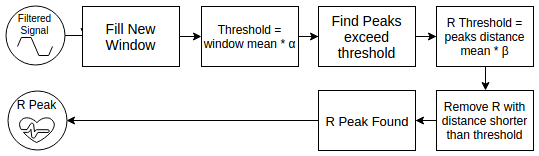
\includegraphics[scale=0.65]{images/processing_modif.png}}
\caption{Processing: Original R Peak Detection}
\label{fig:processing_modif}
\end{figure}

Ket:
$\alpha$ merupakan variabel konstan untuk menaikkan threshold. $n$ menunjukan posisi sampel. $d$ merupakan durasi window, $n$ hingga jumlah sampel pada durasi tersebut. $v_{n}$ merupakan nilai bacaan pada sample ke-$n$.

$\beta$ merupakan variabel konstan untuk menaikkan threshold jarak RR. $i$ menunjukan index peak. $j$ total peak pada window. $r_{n}$ merupakan nilai jarak RR ke-$n$.

\begin{algorithm}[H]
 \begin{algorithmic}[1]
    \Function{peakFinder}{$window, \alpha, d$}
   	\State \text{threshold := $\alpha$ * mean($window, d$)}
	\ForAll{$sample \in window$} 
   	   	\If {$sample > threshold$}
	   		\If {$isPeakArea \neq true$}
	   			\State \text{isPeakArea := true}
				\State \text{tempPeak := sample}
				\State \text{peakCounter += 1}
				\State \text{peaksArea[peakCounter] := tempPeak}
			\ElsIf {$sample > tempPeak$}
				\State \text{tempPeak := sample}
				\State \text{peaksArea[peakCounter] := tempPeak}	
			\EndIf
	   	\Else
	   		\State \text{isPeakArea := false}
   		\EndIf
	\EndFor	
	\State \Return peaksArea
	\EndFunction
 \end{algorithmic}
 \caption{Fungsi Penentuan Peak}\label{Algo:peaksFind}
\end{algorithm} 

\begin{algorithm}[H]
 \begin{algorithmic}[1]
    \Function{falsePeakRemoval}{$peaksArea$}
	\State \text{rThreshold := $\beta$ * mean(distance($peaksArea$))}
	\ForAll{$peak_i \in peaksArea$} 
   	   	\If {$distance(peak_i, peak_{i-1}) < rThreshold$} \Comment{Calculate distance from $peak_i$ to $peak_{i-1}$}
	   		\State $remove(peak, peaksArea)$ \Comment{Remove peak from peak area}
   		\EndIf
	\EndFor	
	\State \Return peaksArea
	\EndFunction
 \end{algorithmic}
 \caption{Prosedur Filter False Peak}\label{Algo:peaksRemove}
\end{algorithm}

\subsection{Algoritma Deteksi Aritmia}
Deteksi Aritmia merupakan salah satu tujuan dari tugas akhir ini. Untuk melakukan deteksi aritmia pada tugas akhir ini menerapkan algoritma usulan Tsipouras (sub bab \ref{bab2_tsipouras}). Algoritma ini dipilih karena kelebihannya yaitu dapat melakukan deteksi hanya menggunakan jarak antar titik R pada data ECG. Karena hanya menggunakan titik R, maka algoritma ini juga dapat secara langsung diterapkan pada data PPG.

\subsection{Visualisasi Gelombang Listrik Jantung}
Pengguna dapat menerima laporan atau melakukan pemantauan pada \textit{dashboard} mereka. Namun untuk menjaga perangkat \textit{dashboard} dapat me-\textit{render} tampilan dengan baik perlu dilakukan penurunan kecepatan sample (lihat gambar \ref{flow:fig_preproc_algorithm}). Selain itu \textit{dashboard} harus terus menerus terkoneksi dengan \textit{Server} untuk bisa mendapatkan data \textit{real-time}. Sehingga kapanpun \textit{server} mendeteksi aritmia pengguna dapat melihat peringatan pada device mereka. 

\begin{figure}[H]
\centering
    %Mulai menggambar Flowchart
\begin{tikzpicture}[node distance=2cm]
\node (start) [cloud] {Start};
\node (get) [io, below of=start] {Input Target FPS};
\node (getFrek) [io, below of=get] {Input Frekuensi Sampel};
\node (counter) [process, below of=getFrek] {counter:= Frek/FPS};
\node (drop) [process, below of=counter] {isDrop:= index mod counter != 0};
\node (dec) [decision, below of=drop] {isDrop?};
\node (send) [process, below of=dec] {Kirim \textit{filtered sample}};
\node (stop) [cloud, below of=send] {Stop};
\draw [arrow] (start) -- (get);
\draw [arrow] (get) -- (getFrek);
\draw [arrow] (getFrek) -- (counter);
\draw [arrow] (counter) -- (drop);
\draw [arrow] (drop) -- (dec);
\draw [arrow] (dec) -- (send);
\draw [arrow] (send) -- (stop);
\draw [arrow] (dec) -- ++(-90pt,0pt) |- (stop);
\end{tikzpicture}
    \caption{Flowchart Rancangan Algoritma Preprocessing}
	\label{flow:fig_preproc_algorithm}
\end{figure}

\subsection{Integrasi Algoritma pada Perangkat Keras}
Tahapan hubungan antara algoritma deteksi dengan perangkat keras digambarkan oleh gambar \ref{seq:fig_detect_algorithm2}. Seorang pasien yang mengenakan \textit{receptor} akan diambil data jantungnya kemudian dikirim ke \textit{server}. Ketika terdeteksi aritmia, \textit{server} akan mengirim \textit{flag} manandakan aritmia terdeteksi ke \textit{dashboard} yang kemudian dilihat oleh pasien, dokter dan keluarga pasien.
\begin{figure}[H]
	\centering
	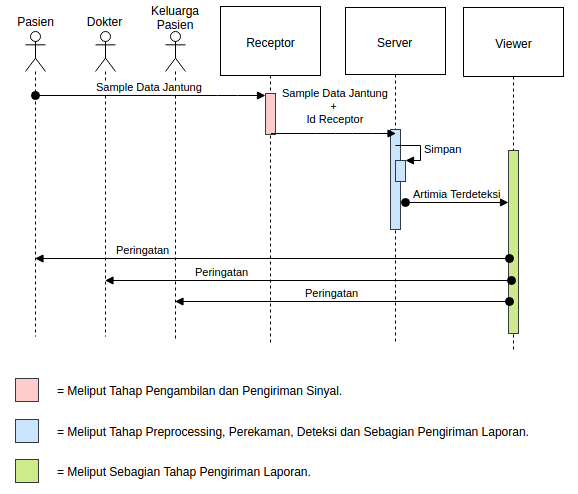
\includegraphics[scale=0.7]{images/sequence1.png}
	\caption{Diagram Tahap (\textit{Sequence}) Algoritma Deteksi}
	\label{seq:fig_detect_algorithm2}
\end{figure}

\section{Skenario Pengujian}
Untuk mengetahui keberahasilan seluruh rancangan diperlukan adanya pengujian, baik secara perangkat maupun algoritma. Hal ini ditujukan mengetahui apakah tujuan tugas akhir ini tercapai.

\subsection{Parameter Pengujian}
Berikut hubungan antara parameter penguji dengan tujuan tugas akhir:

\begin{table}[H]
	\begin{tabular}{|l|L{3cm}|L{2cm}|L{6cm}|}
	\hline
	\rowcolor{gray}
	\textbf{No} & \textbf{Parameter} & \textbf{Tujuan yg Dicakup} & \textbf{Alasan}\\
	\hline
	1 & Jumlah Fitur Sistem & 2, 4 & Mengetahui apakah fitur yang direncanakan bisa berjalan. \\
	\hline
	2 & Delay & 1, 3, 4 & Dengan mengukur \textit{delay} dapat diketahui berapa lama proses pengiriman sehingga dapat diketahui seberapa \textit{Real Time} sistem dapat berjalan. \\
	\hline
	3 & Execution Time & 1, 2, 3, 4 & Dengan mengukur execution time dapat diketahui seberapa banyak sensor yang dapat ditangani oleh spesifikasi server tertentu \\
	\hline
	%4 & FPS & 2, 4 & Dengan mengukur FPS dapat diketahui maksimum FPS agar dapat dijalankan pada banyak \textit{dashboard} \\
	%\hline
	4 & Akurasi & 3 & Dengan mengukur akurasi dapat diketahui seberapa akurat algoritma deteksi yang diterapkan \\
	\hline
	\end{tabular}
\end{table}

\subsection{Konfigurasi Perangkat Keras}
Spesifikasi perangkat keras yang digunakan selama pengujian dapat dilihat pada tabel \ref{tabel:spesifikasi}. Pengujian dilakukan dengan menghubungkan sebuah \textit{receiver}, kepada sebuah \textit{server} dan dipantau oleh 2 \textit{dashboard} (web dan ponsel). Hubungan jaringan perangkat keras digambarkan pada gambar \ref{fig:konfigurasi}.

\begin{table}[H]
	\centering
	\begin{tabular}{|l|L{3cm}|L{8cm}|}
	\hline
	\rowcolor{gray}
	\textbf{No} & \textbf{Perangkat} & \textbf{Spesifikasi} \\
	1 & Receptor &
	\begin{itemize}
		\item ESP-12F
		\item Sensor Pulse
		\item Modul USB TTL CP2102
		\item IC TP4056 LiPo charger
		\item IC LDO regulator RT9193
		\item Battery LiPo protected 180mAh
	\end{itemize} \\
	\hline
	2 & Server & 
	\begin{itemize}
		\item Laptop ASUS A43SD
		\item Intel i3-2350M CPU @ 2.30GHz
		\item RAM DDR3 8GB
	\end{itemize} \\
	\hline
	3 & dashboard Web & 
	\begin{itemize}
		\item Laptop Lenovo G40S
		\item AMD A8 5550M CPU @ 2.1GHz
		\item RAM DDR3 8GB
	\end{itemize} \\
	\hline
	4 & dashboard Android & 
	\begin{itemize}
		\item ZTE A711, Android Lollipop
		\item Snapdragon 615 CPU @ 1.7 GHz
		\item RAM 2GB
	\end{itemize} \\
	\hline
	5 & WiFi Routers & 
	\begin{itemize}
		\item Jetfi G2
		\item WiFi IEEE 802.11b/g/n
	\end{itemize} \\
	\hline
	\end{tabular}
	\caption{Tabel Spesifikasi Perangkat Keras}
	\label{tabel:spesifikasi}
\end{table}

\begin{figure}
	\centering
	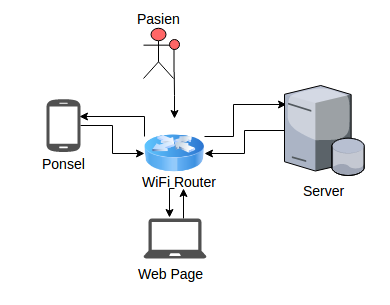
\includegraphics[scale=0.82]{images/konfigurasi.png}
	\caption{Konfigurasi Perangkat Keras}
	\label{fig:konfigurasi}
\end{figure}

\subsection{Pengujian Algoritma Pemantauan}
Sistem tidak bisa dites secara \textit{black box} (memberikan masukkan ke sistem dan melihat hasil) karena pengerjaan tugas akhir tidak didampingi oleh dokter ahli jantung untuk melakukan pengecekan atas hasil deteksi. Sehingga pengujian algoritma dipisah menjadi  2 tahap yaitu, algortima pemantauan dan algoritma deteksi. 

Pengujian algoritma pemantauan dilakukan dengan cara seseorang menggunakan \textit{receiver} dan dilihat keberhasilan pemantauan dari \textit{dashboard}. Pengujian ini ditujukan untuk menguji semua parameter selain parameter 5 (Akurasi).

\subsubsection{a. Delay}
Delay yang diukur ialah waktu tempuh sejak dikirimnya data oleh \textit{receptor} hingga diterima oleh \textit{server}. \textit{Delay} dihitung dengan mengukur rata-rata selisih waktu ($t$) diterimanya data oleh server dikurang dengan waktu kerja sensor ($v$) (persamaan \ref{eq:delay}).

\begin{equation}
Delay = \alpha (\sum_{i=2}^{d} -\frac{(t_{i} - v_{i})}{d})
\label{eq:delay} 
\end{equation}

\subsubsection{b. Execution Time}
\textit{Execution Time} (Waktu eksekusi) diukur pada \textit{receptor} dan \textit{server}. Pada \textit{receptor} \textit{execution time} ialah waktu sejak sampel diambil hingga selesai dikirim ditambah waktu tidur antar sampel, waktu ini disebut sebagai waktu kerja sensor. Pada \textit{server} \textit{execution time} ialah waktu untuk memproses sebuah sampel hingga dimunculkannya sebuah deteksi. Karena pemrosesan dilakukan setiap sebuah \textit{window} terisi, maka \textit{execution time} yang dihitung dengan membagi durasi \textit{window} terhadap dengan jumlah sampel yang diproses (persamaan \ref{eq:exec_time}).

\begin{equation}
ET = (\frac{t_d}{d})
\label{eq:exec_time} 
\end{equation}

%\subsubsection{FPS}
%FPS diukur dengan mecoba konfigurasi \textit{downsample} pada \textit{server} dan melihat tampilan pada \textit{dashboard}.

\subsection{Pengujian Algoritma Deteksi}
Pengujian algoritma deteksi dilakukan dengan memasukkan dataset ECG dari MIT-BIH Arrhythmia Database \cite{mit_bih_paper, mit_bih_web} ke dalam sistem. Untuk mempermudah visualisasi dan analisis data, penulis menjalankan algoritma deteksi pada bahasa pemograman python untuk selanjutnya diimplementasikan ke Node.Js. Pengujian ini ditujukan untuk menguji parameter akurasi.

\subsubsection{a. Dataset}
Dataset dari MIT-BIH \cite{mit_bih_paper, mit_bih_web} terbagi menjadi 48 \textit{records}. Masing masing \textit{record} memiliki panjang 30 menit. Dengan jumlah detak yang berbeda-beda. Rekapitulasi detak yang terekam pada dataset dapat dilihat pada tabel \ref{tabel:dataset}. Setiap \textit{record} telah dianotasi (ditandai) oleh dokter ahli jantung\cite{mit_bih_web}. Rekapitulasi anotasi pada dataset dapat dilihat pada tabel \ref{tabel:result1}  dan \ref{tabel:result2}.

\begin{table}[H]
	\centering
	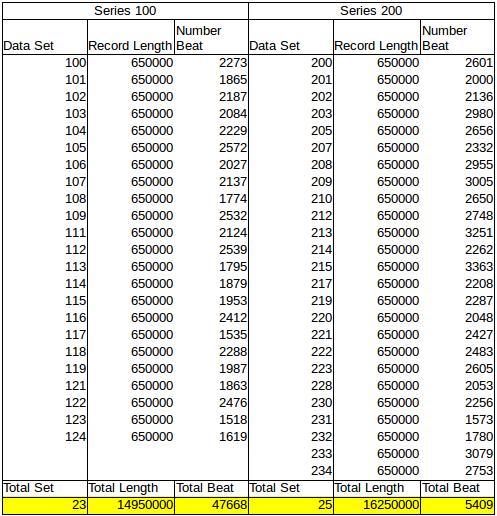
\includegraphics[scale=0.7]{images/tabel_data.png}
	\caption{Tabel Rakapitulasi Jumlah Detak}
	\label{tabel:dataset}
\end{table}	

\begin{table}[H]
	\centering
	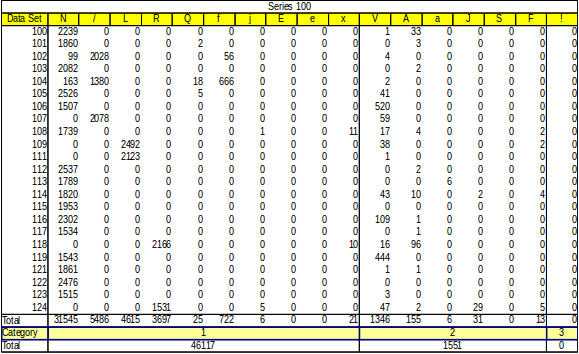
\includegraphics[scale=0.75]{images/result1.png}
	\caption{Tabel Rakpitulasi Aritmia Series 100 dengan Kategori}
	\label{tabel:result1}
\end{table}
\begin{table}[H]
	\centering
	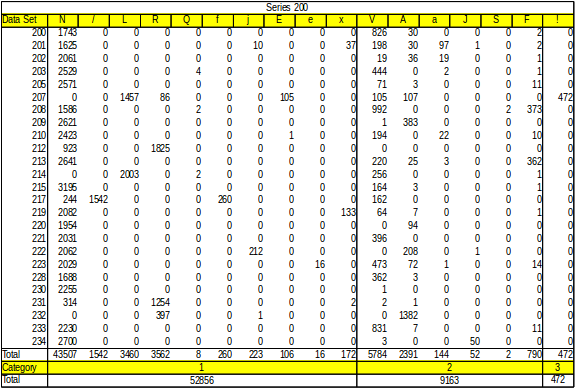
\includegraphics[scale=0.75]{images/result2.png}
	\caption{Tabel Rakpitulasi Aritmia Series 200 dengan Kategori}
	\label{tabel:result2}
\end{table}

\subsubsection{b. Akurasi}
Pengukuran akurasi terbagi menjadi 2 yaitu akurasi deteksi detak dan akurasi deteksi aritmia. Untuk mengukur akurasi jumlah kelas (detak dan aritmia) digunakan persamaan \ref{eq:accuracy}, \ref{eq:specificity} dan \ref{eq:sensitivity}.

\begin{equation}
	Accuracy = \frac{TP + TN}{TP+TN+FP+FN}
	\label{eq:accuracy}
\end{equation}
\begin{equation}
	Specificity = \frac{TN}{TN+FP}
	\label{eq:specificity}
\end{equation}
\begin{equation}
	Sensitivity = \frac{TP}{FN+TP}
	\label{eq:sensitivity}
\end{equation}

\begin{table}[H]
	\centering
	\begin{tabular}{L{3cm}|C{3cm}|C{3cm}|}
	 & \textbf{Predicted: No} & \textbf{Predicted Yes} \\
	\hline
	\textbf{Actual: No} & TN & FP \\
	\hline
	\textbf{Actual: Yes} & FN & TP \\
	\hline	
	\end{tabular}
\end{table}



%
%\chapter{Hasil dan Pembahasan}
\section{Hasil Pengujian}
Setelah melaksanakan pengujian sistem seperti yang telah dibahas pada bab sebelumnya sub bab ini akan memaparkan hasil dari percobaan.
\subsection{Jumlah Fitur Sistem}\label{hasil:jumlahfitur}
%\subsubsection{Pemantauan dan Deteksi}
Pemantauan (aktivitas jantung) dan Deteksi (detak dan aritmia) berhasil dilakukan secara realtime (parameter lainnya, dibahas pada sub bab berikutnya). Berikut perbandingan mode \textit{monitoring} pada sistem di Tugas Akhir ini dengan sistem sejenis lainnya yang berada pada puncak 10 Android Playstore (kata pencarian heart rate) \cite{playstore_heart}.

\begin{table}[H]
	\centering
	\begin{tabular}{|l|L{5cm}|c|L{0.5cm}|L{0.5cm}|L{0.5cm}|L{0.5cm}|L{0.5cm}|L{0.5cm}|L{0.5cm}|L{0.5cm}|}
		\hline
		\rowcolor{gray}
		\textbf{No} & \textbf{Produk} & \textbf{Sen} & \multicolumn{8}{c}{\textbf{Fitur}} \\
		\rowcolor{gray}
		 & & \textbf{sor} & A & B & C & D & E & F & G & H \\
		\hline
		1 & Instant Heart Rate : Heart Rate \& Pulse Monitor & PPG & Y & N & Y & Y & N & Y & N & Y \\
		2 & iCare Health Monitor (BP \& HR) & PPG & Y & N & Y & N & N & Y & N & Y \\
		3 & Heart Rate Monitor(REPS) & PPG & Y & N & Y & Y & N & Y & N & Y \\
		4 & Runtastic Heart Rate Monitor \& Pulse Checker & PPG & Y & N & Y & N & N & Y & N & N \\
		5 & Cardiograph - Heart Rate Meter & PPG & Y & N & Y & Y & N & Y & N & Y \\
		6 & ASUS Heart Rate & PPG & N & N & N & N & N & Y & N & N \\
		7 & Samsung Health & PPG & Y & Y & N & N & N & Y & N & Y \\
		8 & Heart Rate Monitor(Meet Your Need Production) & PPG & N & N & N & N & N & Y & N & N \\
		9 & MobECG & ECG & N & Y & Y & Y & N & Y & N & N \\		
		10 & CMS50Dplus & ECG & N & Y & Y & Y & N & Y & N & N \\
		\hline
		\textbf{*} & \textbf{Tugas Akhir} & \textbf{PPG} & \textbf{Y} & \textbf{Y} & \textbf{Y} & \textbf{Y} & \textbf{Y} & \textbf{Y} & \textbf{Y} & \textbf{Y} \\
		\hline
	\end{tabular}
\end{table}

Ket: \\
A = Identitas User \\
B = Real Time Monitoring \\
C = Melihat Gelombang Jantung \\
D = Merekam Gelombang Jantung \\
E = Multiuser Monitoring \\
F = Deteksi BPM \\
G = Aritmia Alert \\
H = Share Result via Network\\

\subsection{Delay}
Pengujian dilakukan oleh pengguna yang bergerak secara bebas dalam wilayah cakupan router (\textit{receptor}, \textit{router} dan \textit{server} masih dalam satu wilayah) sehingga tidak ada proses routing antara router. Setelah melakukan pengujian sebanyak 3 kali pada waktu berbeda (pagi, siang, malam). Berdasarkan pengujian, didapatkan rata-rata delay percobaan-1 1.60624 ms, percobaan-2 1.36287 ms dan percobaan-3 1.45066 ms. Hasil pengukuran delay tertera pada gambar \ref{fig:delay}. Rata-rata ketiga percobaan ialah 1.47326 ms per sampel.

\begin{figure}[H]
	\centering
	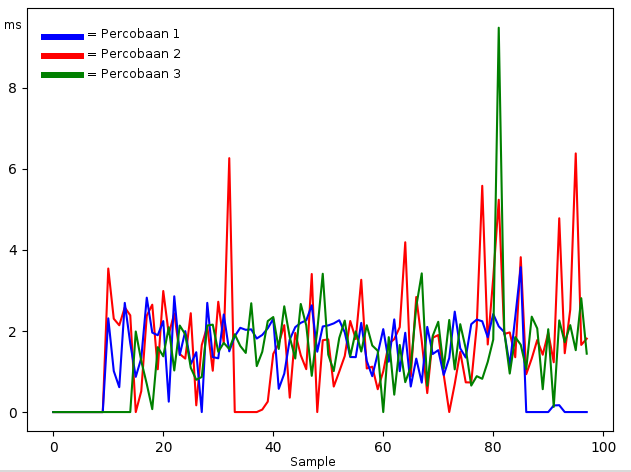
\includegraphics[scale=0.5]{images/delay1.png}
	\caption{Hasil Pengukuran Delay 100 sample}
	\label{fig:delay}
\end{figure}

\subsection{Execution Time}
\textit{Execution Time} perlu diukur pada 2 lokasi yaitu \textit{Receptor} dan \textit{Server}. Hal ini ditujukan untuk mengetahui \textit{maximum sampling speed} yang mungkin dilakukan pada \textit{receptor} sebelum terjadi \textit{bottleneck}. 

Pengujian pada \textit{receptor} dilakukan sebanyak 3 kali pada waktu yang berdekatan (setelah pengujian, \textit{receptor} di \textit{reboot}). Berdasarkan pengujian, didapatkan rata-rata waktu eksekusi percobaan-1 4.36471 ms, percobaan-2 4.74046 ms dan percobaan-3 4.93947 ms. Hasil pengukuran waktu eksekusi tertera pada gambar \ref{fig:exec_time}. Rata-rata ketiga percobaan ialah 4.68155 ms per sampel.

Pengujian pada \textit{server} dilakukan dengan 3 \textit{receptor} yang terhubung (2 + 1 virtual). Berdasarkan pengujian, didapatkan rata-rata waktu eksekusi percobaan-1 0.009496 ms, percobaan-2 0.007823 ms dan percobaan-3 0.008909 ms. Hasil pengukuran waktu eksekusi tertera pada gambar \ref{fig:exec_time2}. Rata-rata ketiga percobaan ialah 0.008742 ms per sampel.

\begin{figure}[H]
	\centering
	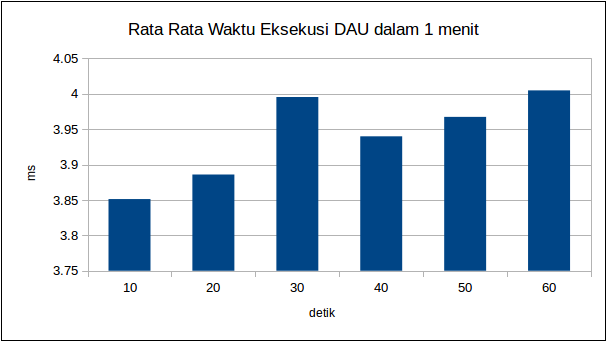
\includegraphics[scale=0.5]{images/exec_time1.png}
	\caption{Hasil Pengukuran Waktu Eksekusi Pada Receptor}
	\label{fig:exec_time}
\end{figure}

\begin{figure}[H]
	\centering
	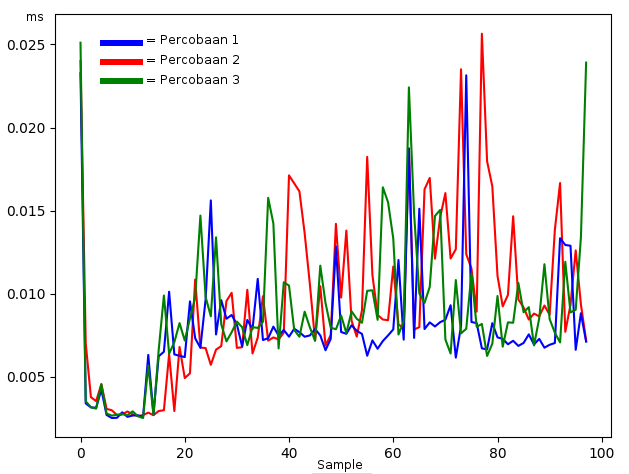
\includegraphics[scale=0.5]{images/exec_time2.png}
	\caption{Hasil Pengukuran Waktu Eksekusi Pada Server}
	\label{fig:exec_time2}
\end{figure}

%\subsection{FPS}
%FPS umumnya ditentukan oleh kapasitas \textit{hardware} yang me-\textit{render} tampilan, namun untuk memaksimalkan jumlah \textit{viewer}, satu nilai FPS perlu dipilih untuk dijalankan pada semua \textit{viewer}. Berikut hasil lengkap percobaan FPS yang dilakukan pada \textit{viewer} web dan android.

%\begin{table}[H]
%	\centering
%	\begin{tabular}{|l|L{4cm}|L{4cm}|}
%	\rowcolor{gray}
%	\textbf{FPS} & \textbf{Web} & \textbf{Android} \\
%	\hline
%	10 & Grafik Patah Patah tapi lancar & Grafik Patah Patah tapi lancar \\
%	\hline
%	20 & Grafik Patah Patah tapi lancar & Grafik halus dan lancar \%\
%	\hline
%	30 & Grafik halus dan sekali kali \textit{freeze} & Grafik halus dan sekali kali \textit{freeze} \\
%	\hline
%	40 & Grafik halus tapi sekali kali \textit{freeze} & Grafik halus tapi sering \textit{freeze} \\
%	\hline
%	50 & Grafik halus tapi sering \textit{freeze} & Grafik halus tapi sering \textit{freeze} \\
%	\hline
%	\end{tabular}
%\end{table}

\subsection{Akurasi}
Setelah melakukan pengujian didapatkan hasil akurasi 94\% untuk detaksi detak dan xx\% untuk deteksi aritmia.
\subsubsection{Akurasi Deteksi Puncak}
Dilakukan percobaan untuk menemukan konfigurasi konstanta deteksi $d$ (durasi window), $\alpha$ (\textit{peak threshold, val by mean}), dan $\beta$ (\textit{min distance threshold, idx by R}). Hasil percobaan dapat dilihat pada tabel \ref{table:exec_time3} dengan variabel eksperimen yang tertera pada tabel \ref{table:experiment_var}. Sedangkan hasil percobaan menggunakan algoritma Pan-Tompkins yang asli dapat dilihat pada tabel \ref{fig:original_pantom}.

\begin{table}[H]
	\centering
	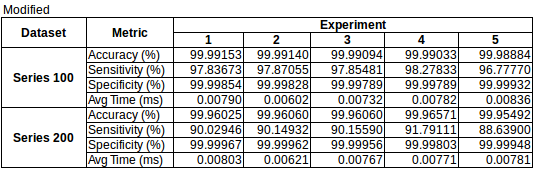
\includegraphics[scale=0.8]{images/modif_beat_detect.png}	
	\caption{Hasil Pengujian Algoritma (Modifikasi) Deteksi Detak Jantung pada Python}
	\label{table:exec_time3}
\end{table}

\begin{table}[H]
	\centering
	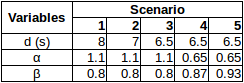
\includegraphics[scale=0.8]{images/experiment_variable.png}
	\caption{Variabel eksperiment}
	\label{table:experiment_var}
\end{table}

\begin{table}[H]
	\centering
	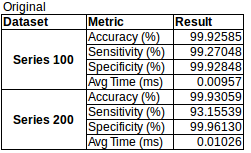
\includegraphics[scale=0.9]{images/original_beat_detect.png}
	\caption{Hasil Pengujian Algoritma (Original) Deteksi Detak Jantung pada Python}
	\label{fig:original_pantom}
\end{table}

Perbandingan antara algoritma modifikasi dengan algoritma pantom yang asli dapat dilihat pada diagram batang \ref{fig:compare_performance_100}, \ref{fig:compare_performance_200} dan \ref{fig:compare_exec}.

\begin{figure}[H]
	\centering
	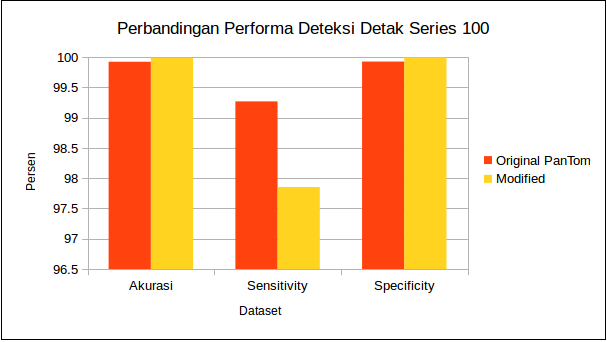
\includegraphics[scale=0.65]{images/beat_perform_100.png}
	\caption{Perbandingan Performa Deteksi Data Series 100}
	\label{fig:compare_performance_100}
\end{figure}
\begin{figure}[H]
	\centering
	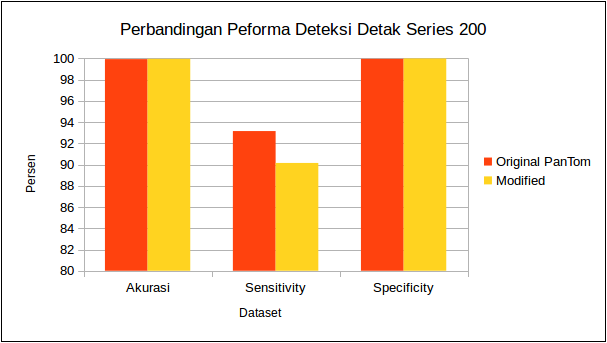
\includegraphics[scale=0.65]{images/beat_perform_200.png}
	\caption{Perbandingan Performa Deteksi Data Series 200}
	\label{fig:compare_performance_200}
\end{figure}
\begin{figure}[H]
	\centering
	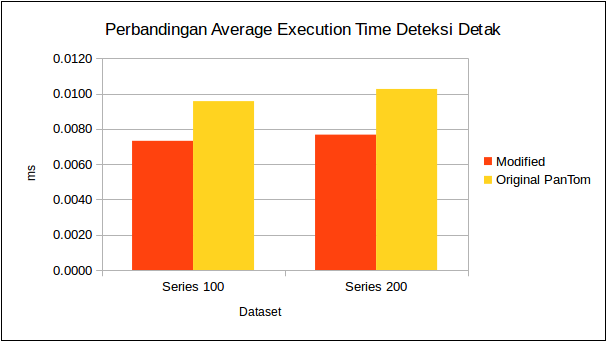
\includegraphics[scale=0.65]{images/beat_exec.png}
	\caption{Perbandingan Waktu Akurasi}
	\label{fig:compare_exec}
\end{figure}

\subsubsection{Akurasi Deteksi Aritmia}
Pengujian akurasi deteksi aritmia terbagi menjadi 3 bagian. Pengujian pertama, sistem deteksi menerima inputan detak jantung asli sesuai data dari MIT BIH. Pengujian kedua, sistem deteksi menerima inputan detak jantung hasil deteksi tahap sebelumnya dengan algoritma asli dari PanTomkins. Pengujian ketiga, sistem deteksi menerima inputan detak jantung hasil deteksi tahap sebelumnya dengan algoritma modifikasi dari PanTomkins. Hasil perbandingan pengujian dapat dilihat pada gambar \ref{fig:aritmia_accuracy}, \ref{fig:aritmia_sensitivity}, dan \ref{fig:aritmia_specificity}.

\begin{table}[H]
	\centering
	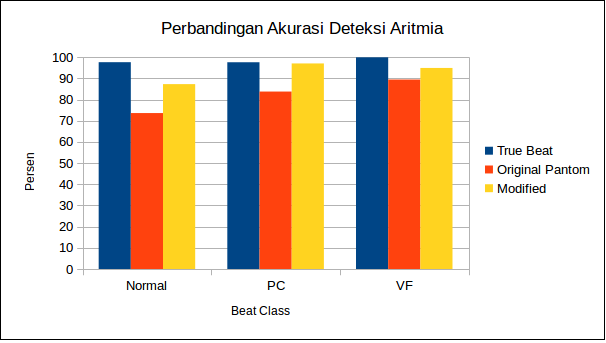
\includegraphics[scale=0.7]{images/aritmia_acc.png}
	\caption{Perbandingan akurasi deteksi Aritmia dengan input berbeda}
	\label{fig:aritmia_accuracy}
\end{table}
\begin{table}[H]
	\centering
	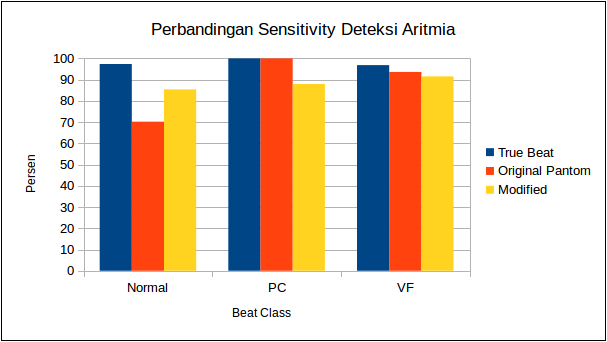
\includegraphics[scale=0.7]{images/aritmia_se.png}
	\caption{Perbandingan sensitvitas deteksi Aritmia dengan input berbeda}
	\label{fig:aritmia_sensitivity}
\end{table}
\begin{table}[H]
	\centering
	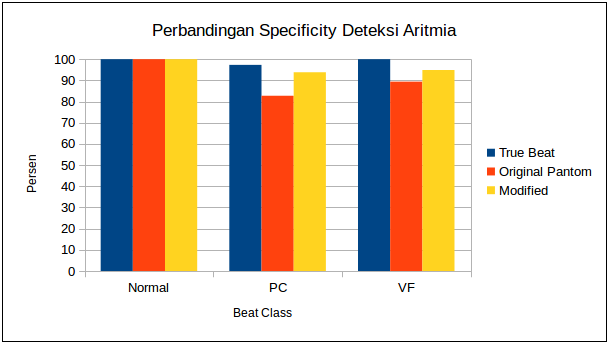
\includegraphics[scale=0.7]{images/aritmia_sp.png}
	\caption{Perbandingan spesifisitas deteksi Aritmia dengan input berbeda}
	\label{fig:aritmia_specificity}
\end{table}

\section{Pembahasan}
Dengan pengimplementasian rancangan arsitektur, sistem yang dibangun dapat memiliki semua fitur yang dimiliki sistem sejenis (\ref{hasil:jumlahfitur}). Delay yang terjadi selama pengiriman sampel selalu berubah ubah namun memiliki rata rata 1.47326 ms. Perubahan nilai delay terjadi karena pengaruh kehandalan jaringan (WiFi) dan subjek yang bebas bergerak. 

Waktu eksekusi diukur pada \textit{receptor} dan \textit{server}. Pada \textit{receptor} terlihat waktu eksekusi yang berubah ubah, ini dipengaruhi oleh adanya \textit{interupt} pengambilan sampel, pembuatan dan pengiriman paket, dan \textit{buffer memory management}. Sebagai perbandingan, tanpa melakukan pengiriman waktu eksekusi hanya selama 0.001 ms (waktu untuk mengambil sampel). Karena rata rata waktu eksekusi pada \textit{receptor} ialah 4.68 ms maka maksimum frekuensi sampel ialah 200Hz, atau setara dengan 1 sampel/5ms. 

Sedangkan pada \textit{server}, terlihat waktu eksekusi sangat tinggi pada permulaan kemudian sangat rendah lalu berfluktuasi, hal ini disebabkan oleh server yang membutuhkan waktu lebih lama untuk memulai \textit{subprocess} untuk tiap \textit{receptor} yang terhubung. Kemudian, tiap proses hanya mengisi buffer hingga cukup untuk dilakukan operasi deteksi. Penggunaan Node.JS sebagai server juga memberikan dampak dalam kecepatan. Dibandingkan dengan Python, Node.JS dapat bekerja hampir 3 kali lebih cepat (gambar \ref{table:exec_time3}). Karena maksimum frekuensi sampel yang dapat diterapkan ialah 1 sampel tiap 5ms dan waktu eksekusi 1 sampel ialah 0.008742 ms maka secara matematis server dapat memproses sekitar 570 device secara bersamaan (maksimum total sensor dan dashboard yang terhubung, 5ms / 0.008742ms).

Pada segi performansi, algortima deteksi puncak R terlihat hasil modifikasi menghasilkan akurasi, \textit{specificity} dan \textit{sensitivity} yang hampir menyamai algoritma pantomkins yang asli bahkan cenderung lebih baik (kecuali sensitivity). Hal ini secara langsung berdampak pada performa algoritma deteksi aritmia yang diterapkan sehingga menghasilkan tren performa yang sama (lebih rendah pada paramater sensitivity).

%
%\chapter{Kesimpulan dan Saran}
\section{Kesimpulan}

\section{Saran}
Berdasarkan proses perancangan dan pengujian sistem, penulis melihat beberapa pengembangan rancangan dan langkah pengujian yang dapat dilakukan, antara lain:
\begin{enumerate}
	\item Bekerjasama dengan dokter ahli jantung untuk melakukan pengujian nyata
	\item Memilih fitur dan klasifikasi lain untuk meningkatkan kehandalan akurasi deteksi	
	\item Melakukan simulasi jaringan \textit{unreliable} dengan menggunakan WANem[xx]. Hal ini ditujukan agar dapat menguji kehandalan sistem jika diterapkan di dunia nyata.
	\item Merancang \textit{receptor} yang lebih hemat daya,
	\item Merancang \textit{Device Interface} dan \textit{Application Programming Iterface} (API) sehingga sistem dapat menerima input dari perangkat yang telah tersedia dipasaran.
\end{enumerate}
%
\cleardoublepage
\addcontentsline{toc}{chapter}{Daftar Pustaka}
\bibliographystyle{acm} %harvard style
\bibliography{References}
%
%\pagebreak
\cleardoublepage
\addcontentsline{toc}{chapter}{Lampiran}
\chapter*{Lampiran}

\section{Koefisien Proses Filter}\label{lampiran:bandpass}
\begin{table}[htbp]
	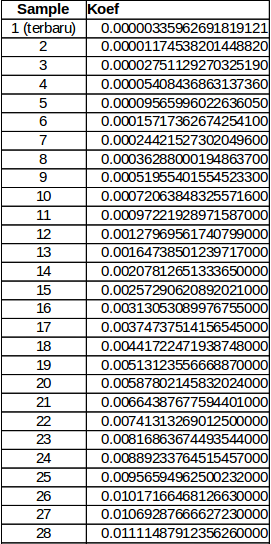
\includegraphics[scale=0.6]{images/koef1.png}
	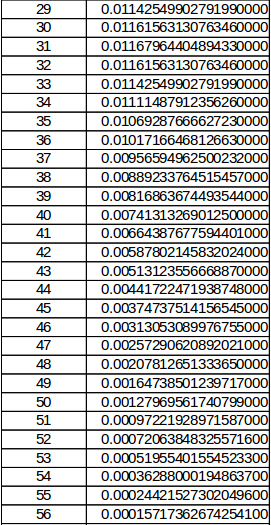
\includegraphics[scale=0.6]{images/koef2.png}
	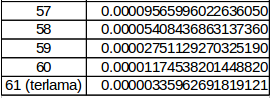
\includegraphics[scale=0.6]{images/koef3.png}
	\caption{Daftar Koefisien Band Pass Filter}
\end{table}
\begin{table}[htbp]
	\centering
	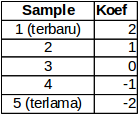
\includegraphics[scale=0.8]{images/koef4.png}
	\caption{Daftar Koefisien Derivative Filter}
\end{table}
\end{document}
